\apendice{Especificación de diseño}

\section{Introducción}

A continuación presentaremos los diseños que se elaborado para poder realizar los objetivos anteriores. Se ha incluido el diseño de datos, el diseño procedimental y el diseño arquitectónico.

\section{Diseño de datos}

La estructura de datos presentada en este proyecto se recoge en una base de datos relacional \textit{MySQL}. En un primer momento se construyó el diagrama entidad relación a través del cual se obtuvo el diagrama relacional. En las figuras~\ref{img:modeloER} y~\ref{img:modeloRelacional} presentamos los modelos entidad relación y relacional respectivamente.

A continuación se describirán cada una de las entidades:

\begin{itemize}
	
	\item \textit{countries}: Los países presentes en nuestra instalación.
	
	\item \textit{regions}: Cada una de las regiones pertenecientes a un país.
	
	\item \textit{arcs}: Comunicación entre dos regiones.
	
	\item \textit{fuels}: Tipos de aceites.
	
	\item \textit{technologies}: Tipos de tecnologías renovables y no renovables.
	
	\item \textit{typelines}: Tipo de conexión de los arcos entre dos regiones.
	
	\item \textit{arcs\_typelines}: Relación entre el arco y el tipo de arco.
	
	\item \textit{fuels\_technologies}: Relación entre el aceite y la tecnología.
	
	\item \textit{regions\_technologies}: Relación entre la región y qué tecnología hay presente.
	
	\item \textit{rangedemands}: Datos de demanda en un instante de tiempo concreto.
	
	\item \textit{rangemeteos}: Datos meteorológicos en un instante de tiempo concreto.
	
	\item \textit{rangerenowables}: Datos de fuentes renovables en un instante de tiempo concreto.

\end{itemize}

\begin{figure}[h]
	\centering
	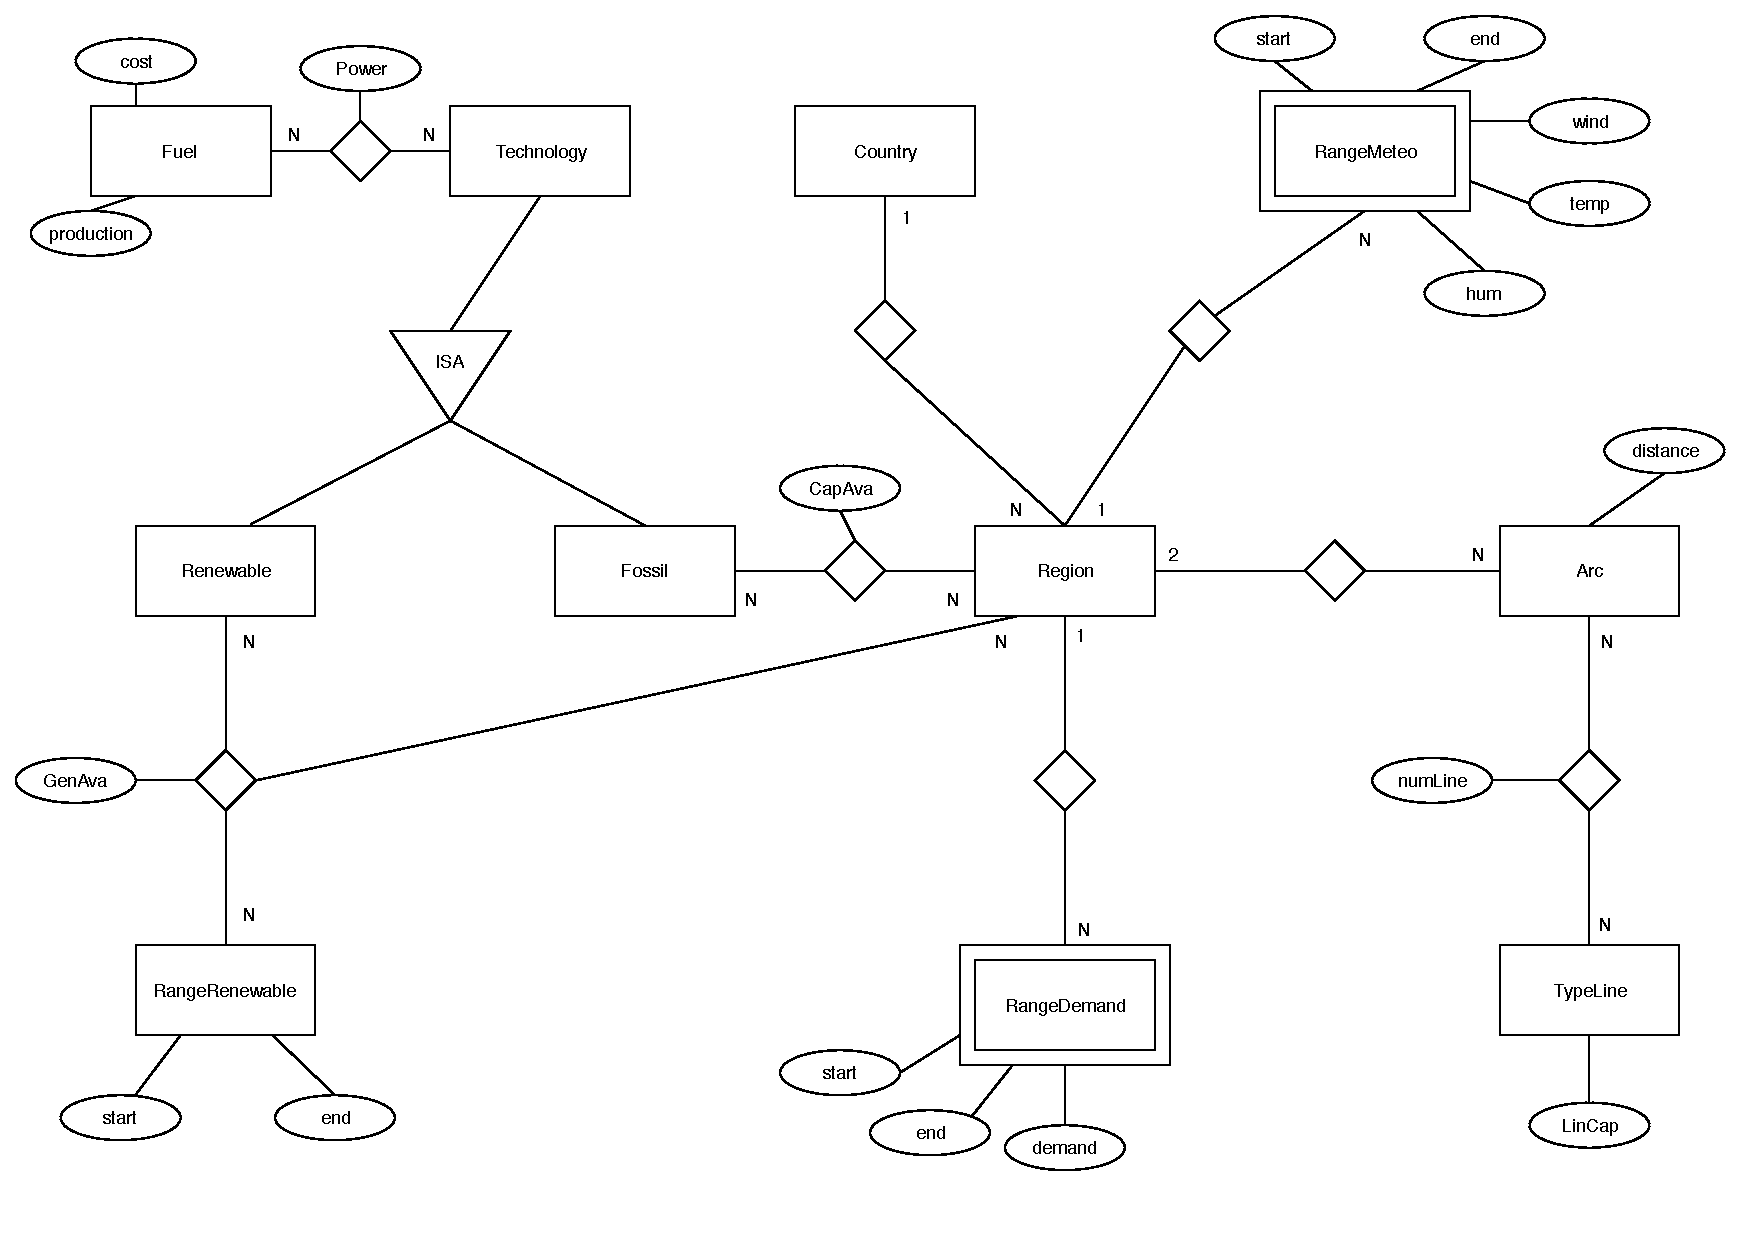
\includegraphics[width=1\textwidth]{/anexos/Diseno/DiagramaER}
	\caption{Diagrama entidad relación.}
	\label{img:modeloER}
\end{figure}

\begin{figure}[h]
	\centering
	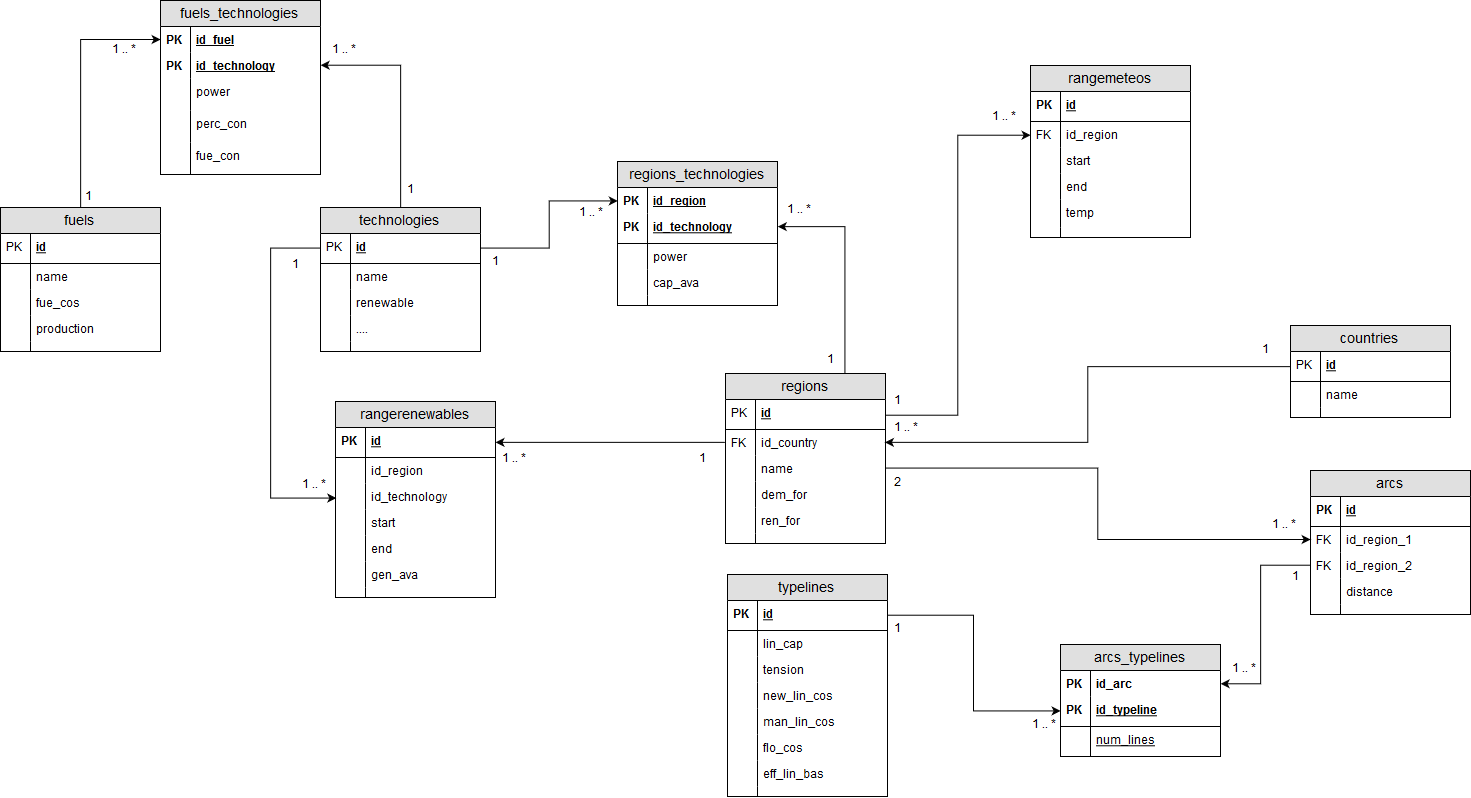
\includegraphics[width=1\textwidth]{/anexos/Diseno/DiagramaRelacional}
	\caption{Diagrama relacional.}
	\label{img:modeloRelacional}
\end{figure}

\newpage


\section{Diseño procedimental}

En esta sección se realizará un diagrama de secuencia del caso de uso 1 que representa la actualización de datos mediante formularios. Concretamente, se representará la edición de una región. Podemos ver el diagrama de secuencia en la figura~\ref{img:modeloSecuencial}.

\begin{figure}[h]
	\centering
	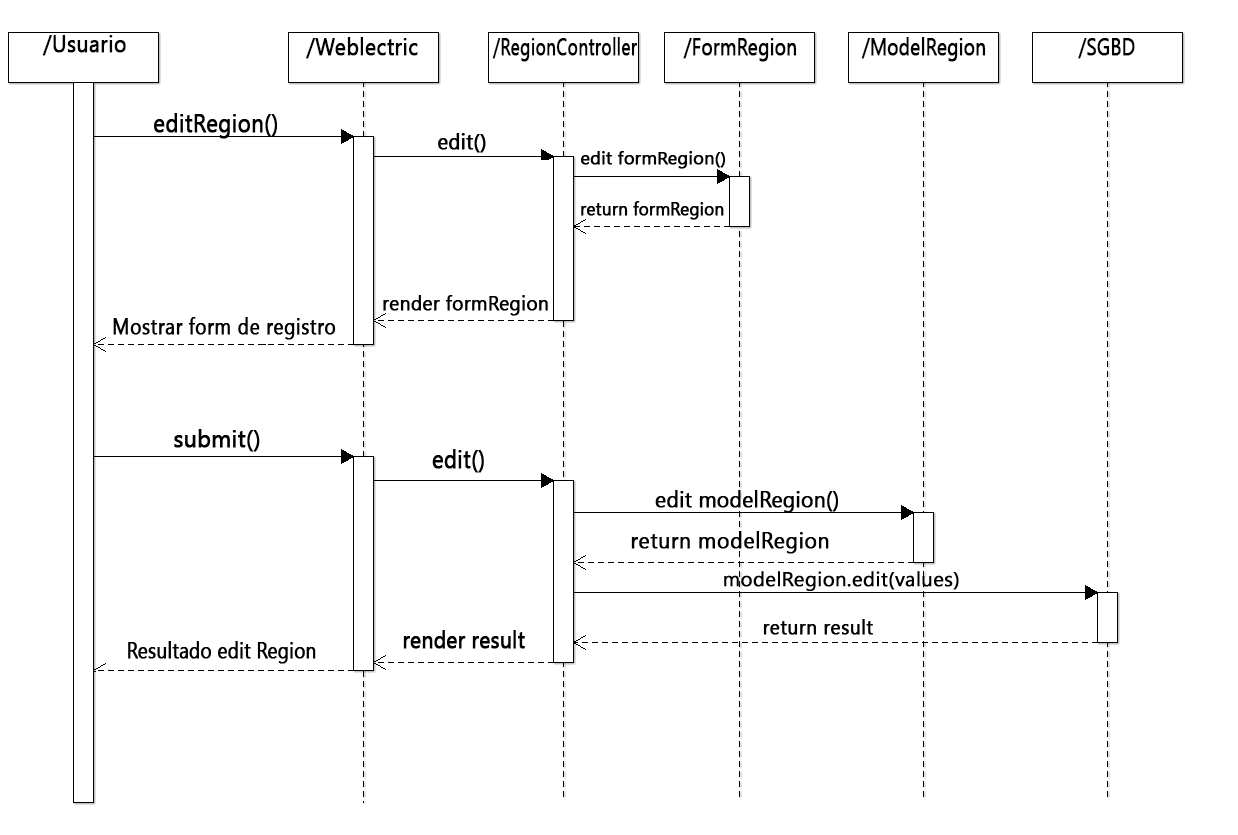
\includegraphics[width=1\textwidth]{/anexos/Diseno/DiagramaSecuencial}
	\caption{Diagrama secuencial.}
	\label{img:modeloSecuencial}
\end{figure}

\newpage

\section{Diseño arquitectónico}

En este apartado se va a comentar como está diseñada la aplicación.

Para el diseño de \textit{Weblectric} se ha seguido un patrón Modelo-Vista-Controlador~\ref{img:mvc}. Mediante este patrón, la aplicación queda completamente estructurada en tres secciones:

\begin{itemize}
	
	\item \textit{Modelo:} Se destinan a esta parte todas las funciones de interacción directa con la base de datos.
	
	\item \textit{Vista:} Aquí guardamos las pantallas que interactúan con el cliente.
	
	\item \textit{Controlador:} Aquí encontramos lo que es la lógica de la aplicación. Hace de unión entre la vista y el modelo.

\end{itemize}

En la tabla~\ref{tabla:estructuraMVC} podemos ver que directorio corresponde en nuestro proyecto a cada una de estas tres grandes secciones.

\begin{table}[h]
	\centering
	\caption{Estructura MVC en \textit{Weblectric}.}
	\label{tabla:estructuraMVC}
	\rowcolors {2}{gray!20}{}
	\begin{tabular}{p{5cm} p{5cm}}
		\toprule
		Patrón MVC 					 & Directorio en \textit{Weblectric}  \\ \midrule
		Modelos			        	 & \textit{models} 			    \\ 
		Vistas						 & \textit{templates}		    \\
		Controladores          		 & \textit{controllers}		 	\\ \bottomrule
	\end{tabular}
\end{table}

\begin{figure}[h]
	\centering
	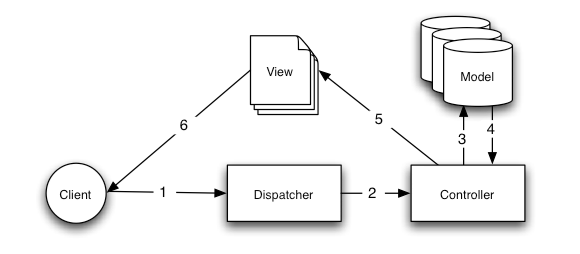
\includegraphics[width=1\textwidth]{/anexos/Diseno/mvc}
	\caption{Patrón Modelo-Vista-Controlador.~\cite{img:MVC}}
	\label{img:mvc}
\end{figure}

\newpage

Una vez conocida la estructura de la aplicación, mostraremos los pasos seguidos para construir las vistas. Dividiremos la clasificación en dos grupos: la idea inicial elaborada a través de unos \textit{mockups} y el resultado final.

\subsection{Mockups} 

El primer paso fue diseñar una plantilla (\textit{layout}). Esta plantilla, que podemos ver en la figura~\ref{img:layout} es común a todas las vistas.

Posteriormente, pasamos a diseñar la pantalla principal~\ref{img:home}. Aquí se iban a listar todas las entidades para que el usuario pudiese acceder a administrarlas.

Como se puede ver en la figura~\ref{img:home}, al pasar el ratón por encima, aparecerá una pequeña animación diferenciando cada una de las entidades. La siguiente pantalla que vamos a presentar es la administración. Tenemos dos tipos de administraciones, las que son a partir de formularios y las que son mediante la subida de una hoja de cálculo. Pulsando en una de las entidades, nos iremos a su pantalla principal, a cada entidad la que le corresponda. 

\subsubsection{Administración mediante formularios} 

En la figura~\ref{img:entidadHome}, podemos ver la pantalla de administración de las entidades que utilizan formularios. En esta vista podremos hacer las siguientes acciones:

\begin{itemize}
	\item Crear un nuevo elemento:~\ref{img:entidadNew}.
	\item Editar un elemento existente:~\ref{img:entidadEdit}.
	\item Visualizar detalles de un elemento existente:~\ref{img:entidadView}.
	\item Eliminar un elemento:~\ref{img:entidadDelete}.
\end{itemize}

\subsubsection{Administración mediante hojas de cálculo} 

Como ya hemos comentado, hay algunas entidades que se administran a través de hojas de cálculo. En la figura~\ref{img:entidadExcel} encontramos un ejemplo. Además, existe la posibilidad de poder descargar una plantilla con todos los datos actuales, podemos modificar los datos y subir el fichero. 

\newpage

\subsection{Resultado final} 

Una vez presentados los mockups, comentaremos los cambios que se han ido produciendo a raíz de proposiciones del cliente y mejoras personales que hemos ido realizando durante el desarrollo.

La plantilla de la aplicación ha sufrido modificaciones pues además de añadir un logotipo personalizado para \textit{Weblectric}, se ha tenido que incluir una nueva funcionalidad, un botón para restablecer la base de datos a su situación inicial. Estos cambios se contemplan en la figura~\ref{img:Flayout}.

Sin embargo, el cambio más significativo viene dado en la pantalla principal. Una vez enseñado el resultado al cliente, nos mandó reestructurar la forma en que distribuimos cada una de las entidades. Actualmente, ya no se representan así, sino que existen diferentes agrupaciones, cada una con su color y animación identificativos.

La estructura de la aplicación, con los cambios aplicados, queda de la siguiente manera:

\begin{itemize}
	
	\item Un primer grupo con tres pestañas~\ref{img:Fhome}:
	
	\begin{itemize}
		
		\item Countries data: \ref{img:Fcountries}. 
		
		\begin{itemize}
			
			\item Country.
			\item Renewable source.
			\item Climate.
			\item Current System.
			
		\end{itemize}
		
		\item Technologies:\ref{img:Ftechnologies}.
		
		\begin{itemize}
			
			\item Generation technologies.
			\item Types of lines.
			\item Fuels.
			
		\end{itemize}
		
		\item Simulation: \ref{img:Fsimulation}.
		
		\begin{itemize}
			
			\item Objectives.
			\item Scenarios.
			\item Download.
			
		\end{itemize}
		
	\end{itemize}
	
\end{itemize}

A continuación, siguiendo con el mismo criterio que en el apartado de los \textit{mockups}, mostraremos las imágenes clasificando los dos tipos de administraciones

\subsubsection{Administración mediante formularios} 

Cogiendo como ejemplo la entidad "technologies", los resultados son: 

\begin{itemize}
	\item Pantalla principal de esa entidad~\ref{img:FentidadHome}.
	\item Crear una nueva tecnología:~\ref{img:FentidadNew}.
	\item Editar una tecnología:~\ref{img:FentidadEdit}.
	\item Visualizar detalles de una tecnología:~\ref{img:FentidadView}.
	\item Eliminar una tecnología:~\ref{img:FentidadDelete}.
\end{itemize}

\subsubsection{Administración mediante hojas de cálculo} 

En la figura~\ref{img:FentidadExcel} encontramos un ejemplo de como se administran los datos climáticos. 

%MOCKUPS:

\begin{figure}[h]
	\centering
	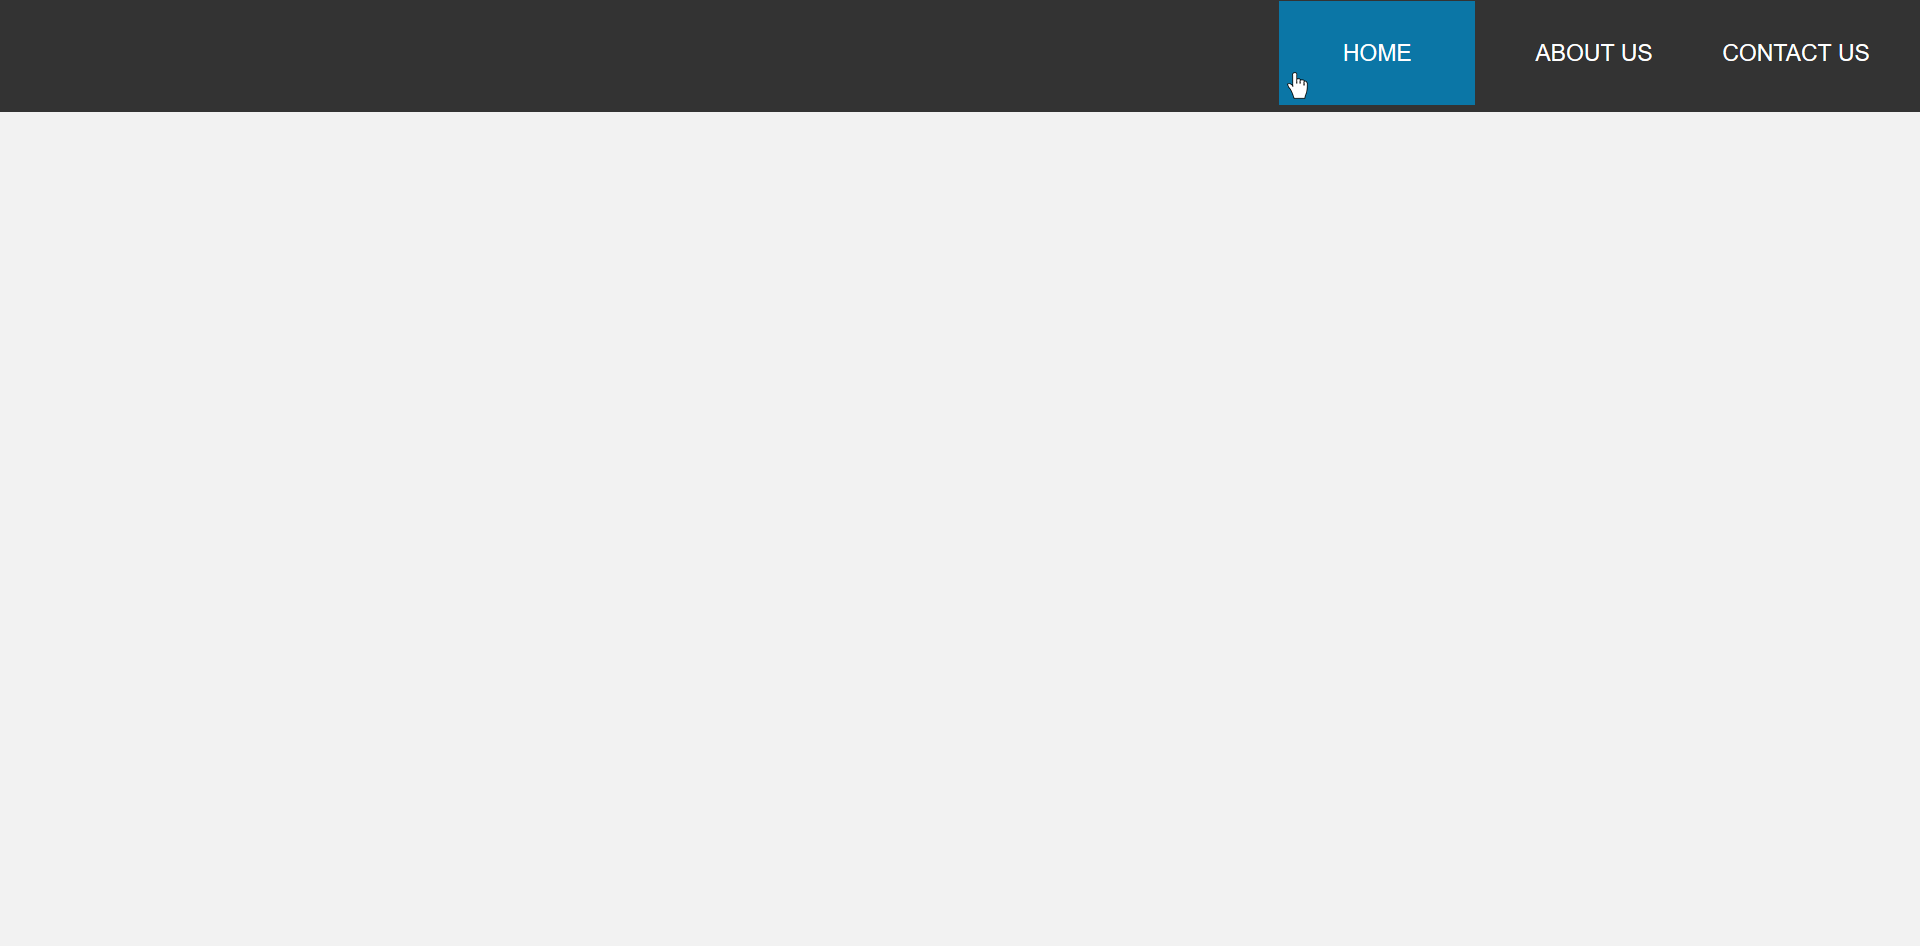
\includegraphics[width=1\textwidth]{/anexos/Diseno/Mockups/layout}
	\caption{Mockup: Plantilla común a todas las vistas.}
	\label{img:layout}
\end{figure}

\begin{figure}[h]
	\centering
	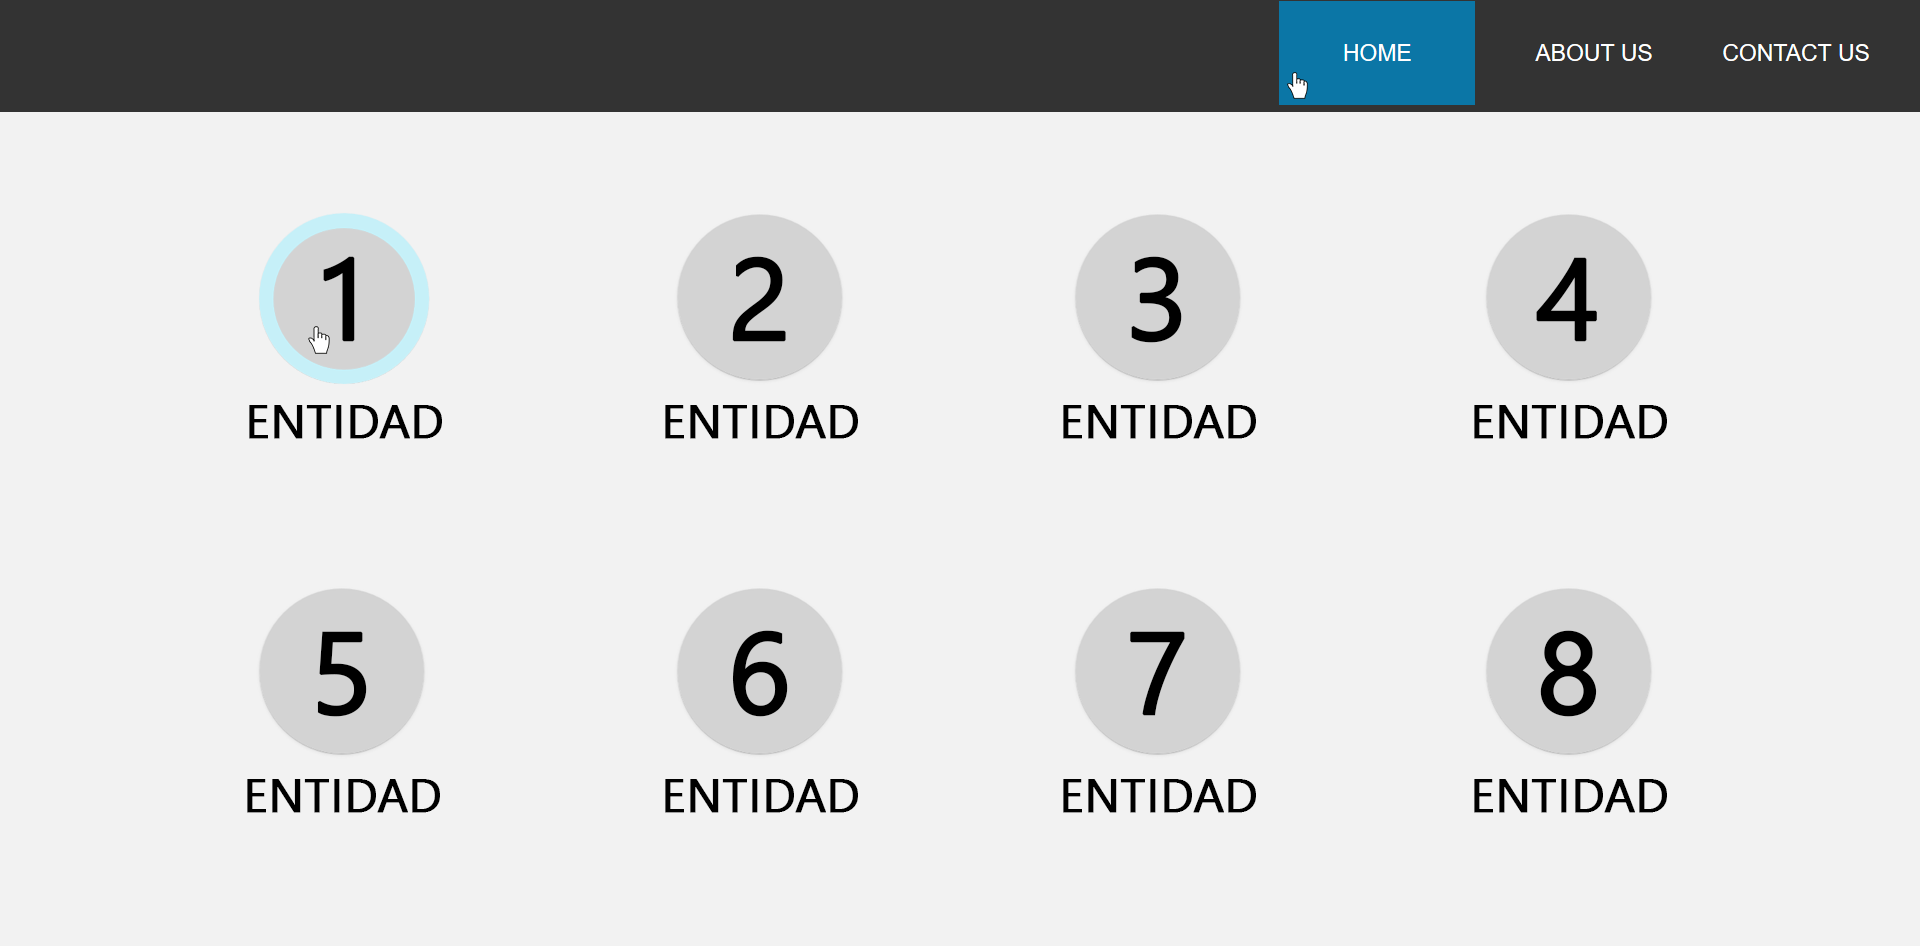
\includegraphics[width=1\textwidth]{/anexos/Diseno/Mockups/home}
	\caption{Mockup: Pantalla principal.}
	\label{img:home}
\end{figure}

\begin{figure}[h]
	\centering
	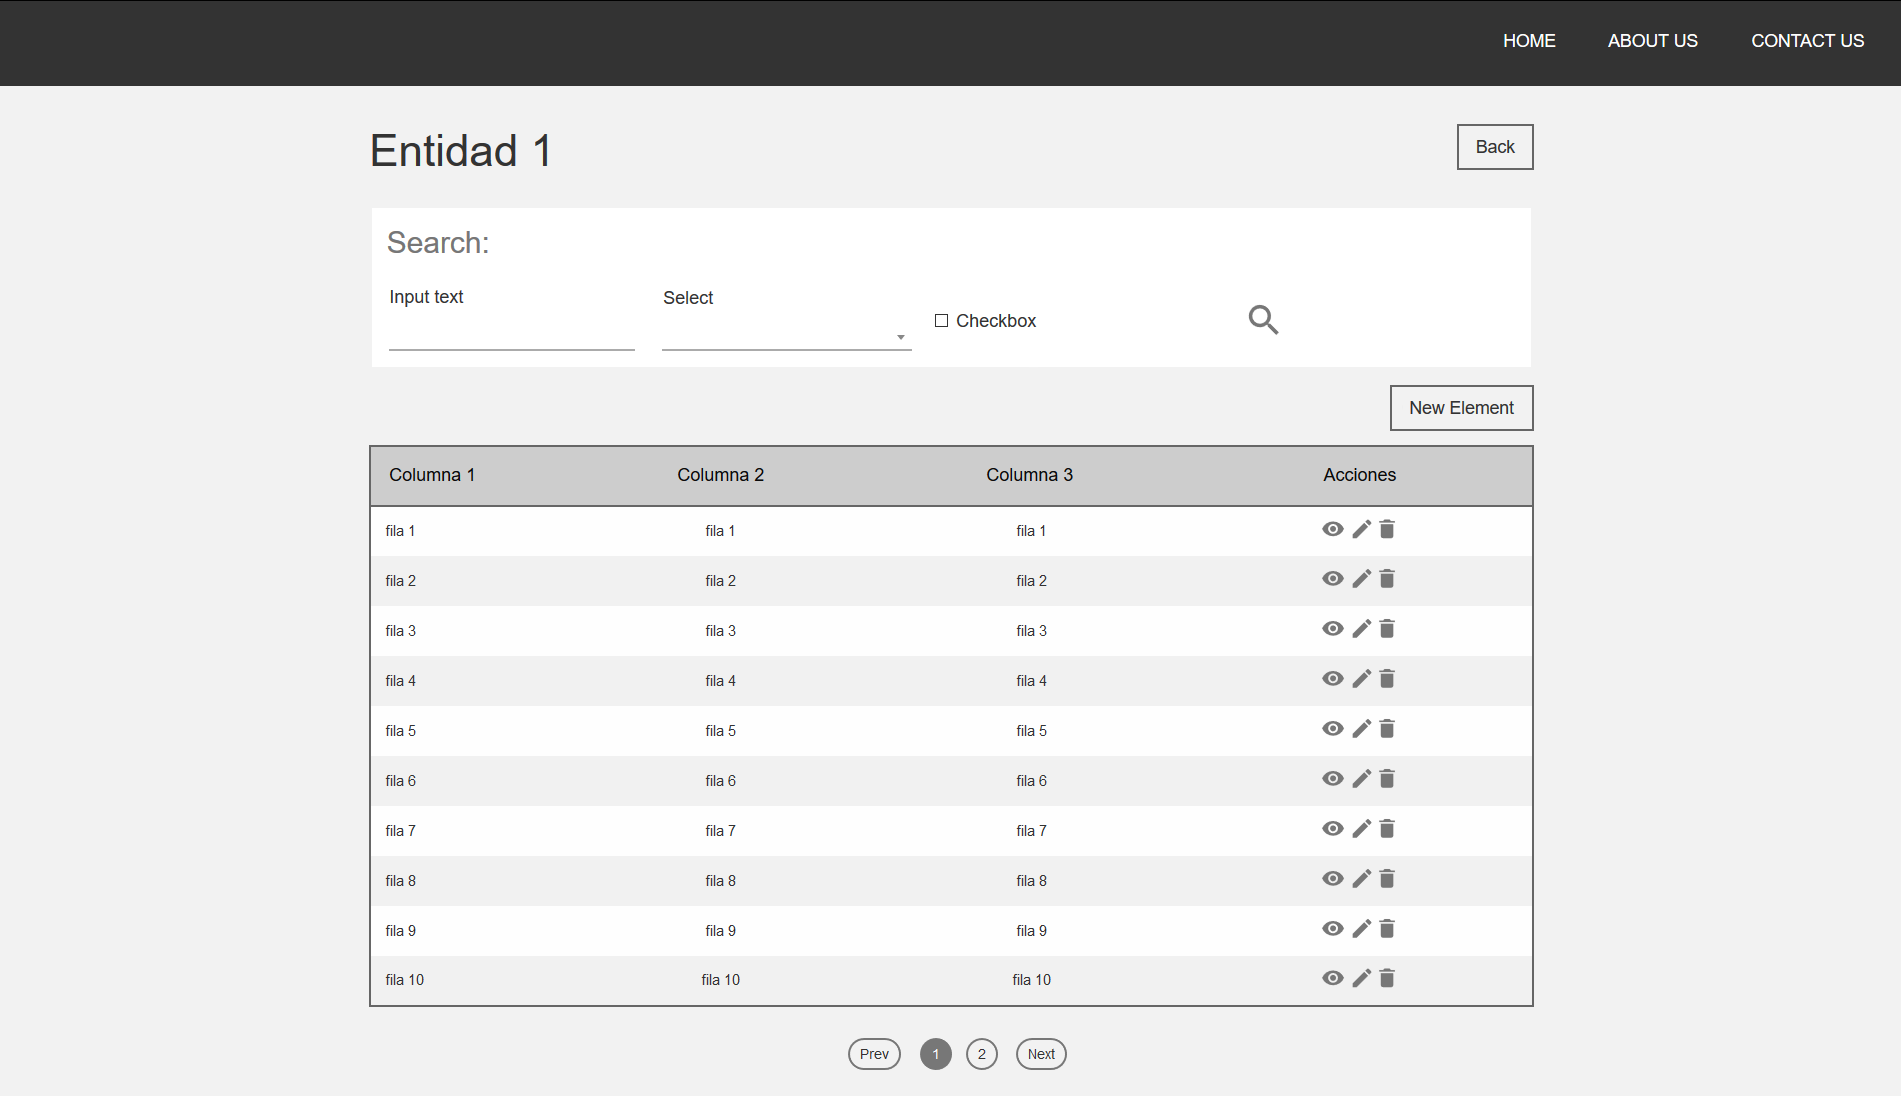
\includegraphics[width=1\textwidth]{/anexos/Diseno/Mockups/entidadHome}
	\caption{Mockup: Pantalla principal de la entidad 1.}
	\label{img:entidadHome}
\end{figure}

\begin{figure}[h]
	\centering
	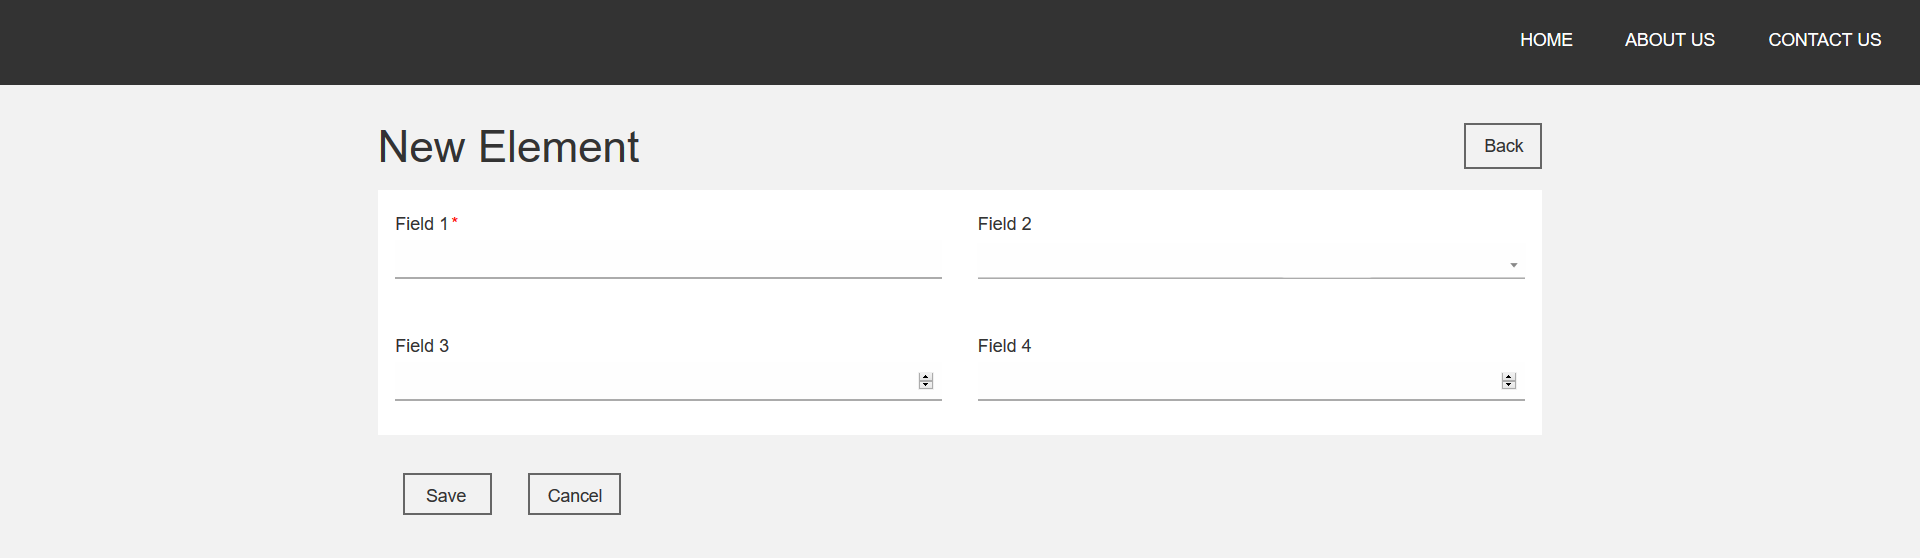
\includegraphics[width=1\textwidth]{/anexos/Diseno/Mockups/entidadNew}
	\caption{Mockup: Alta de un elemento.}
	\label{img:entidadNew}
\end{figure}

\begin{figure}[h]
	\centering
	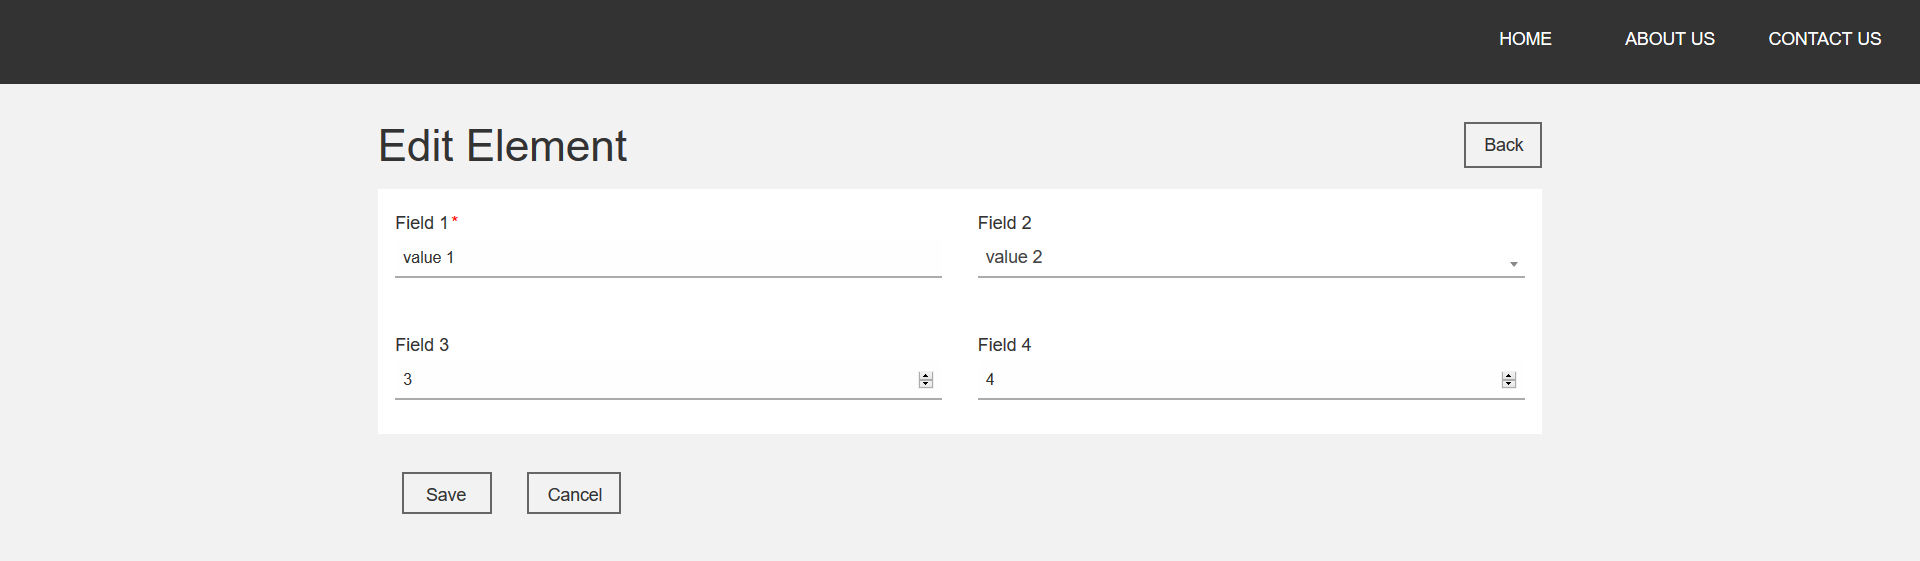
\includegraphics[width=1\textwidth]{/anexos/Diseno/Mockups/entidadEdit}
	\caption{Mockup: Edición de un elemento.}
	\label{img:entidadEdit}
\end{figure}

\begin{figure}[h]
	\centering
	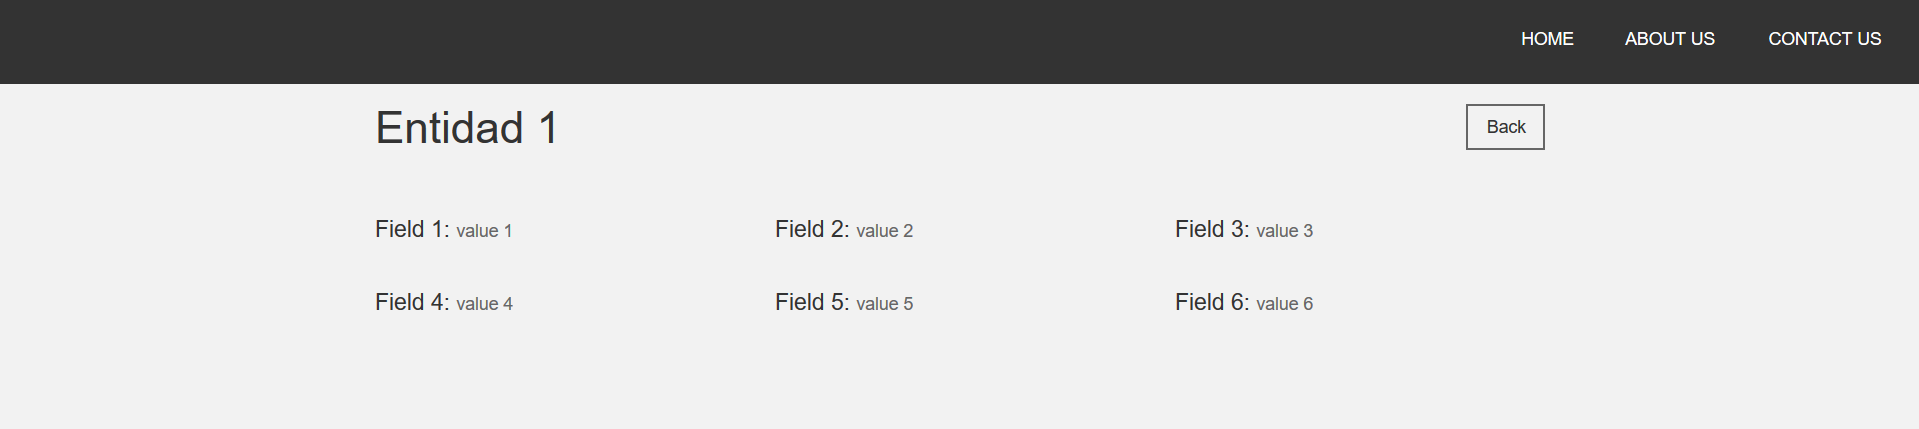
\includegraphics[width=1\textwidth]{/anexos/Diseno/Mockups/entidadView}
	\caption{Mockup: Visualización completa de un elemento.}
	\label{img:entidadView}
\end{figure}

\begin{figure}[h]
	\centering
	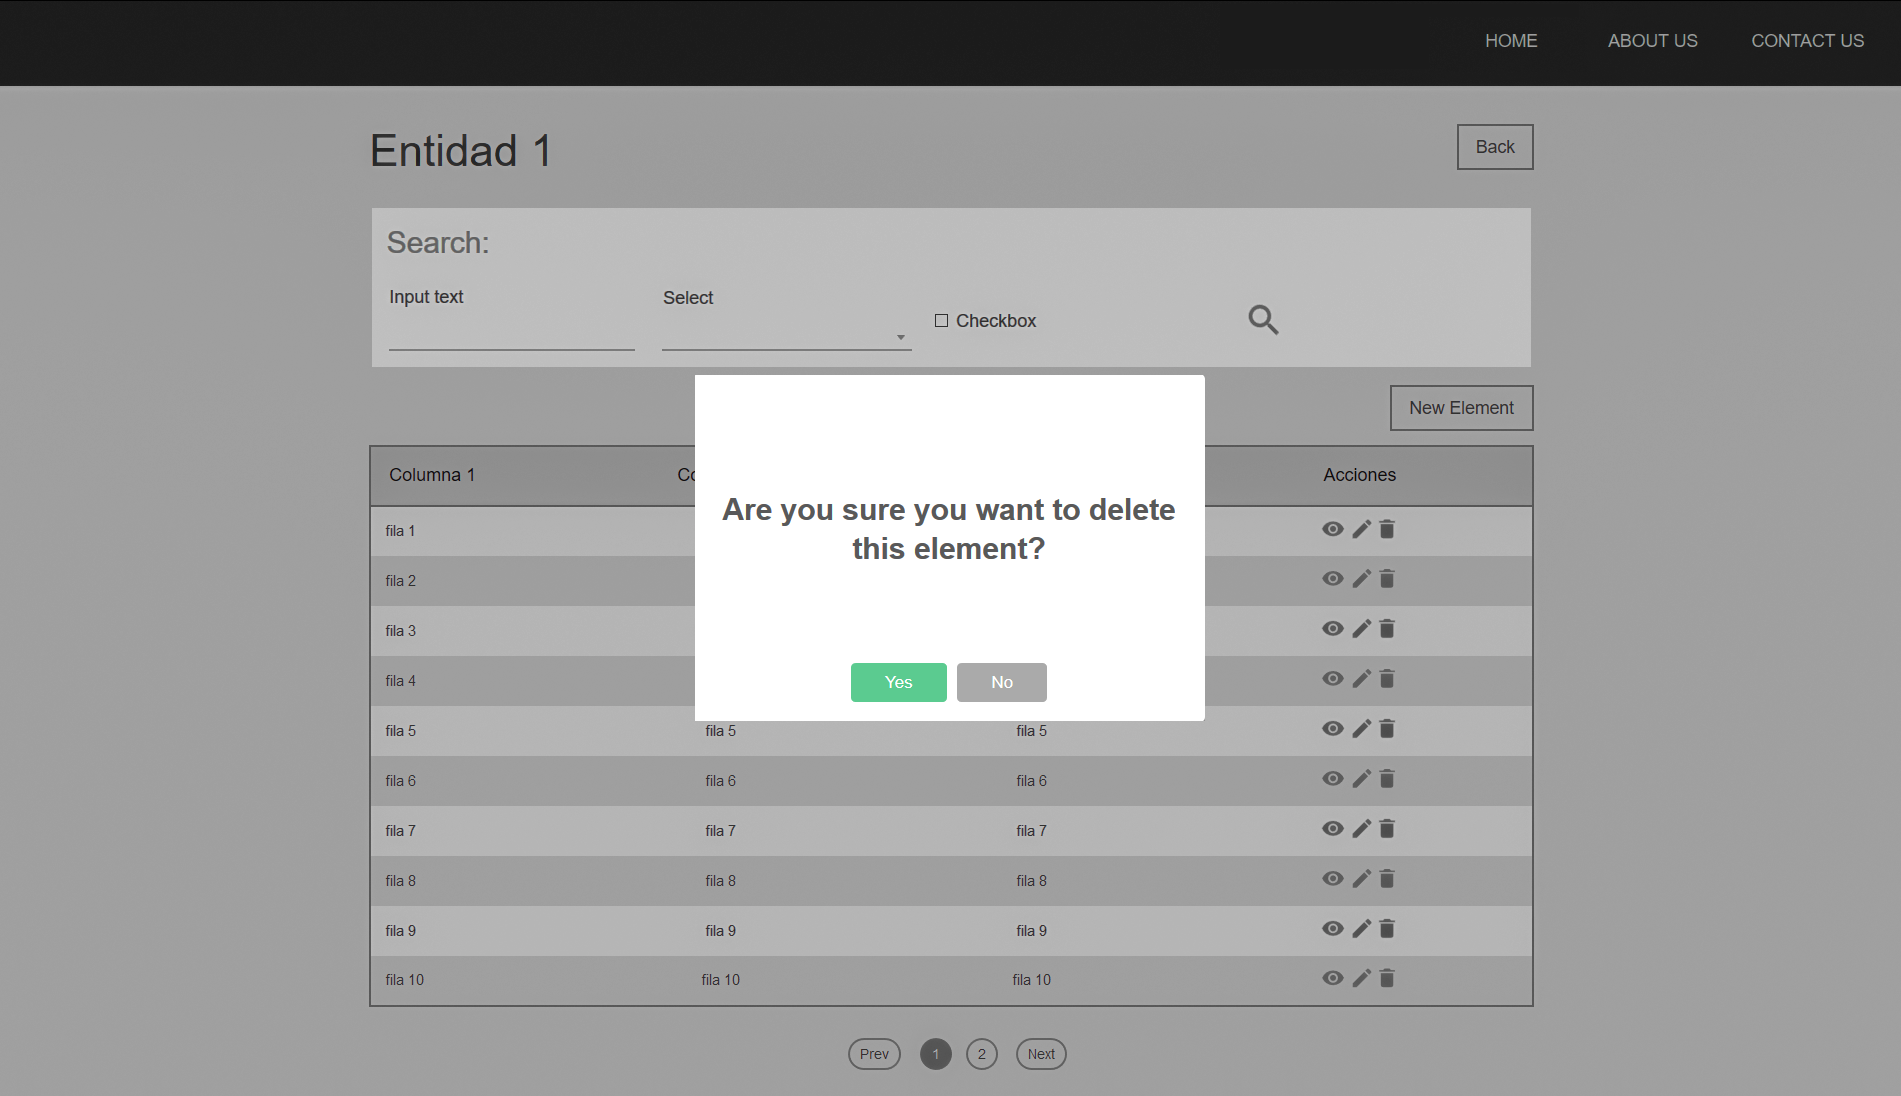
\includegraphics[width=1\textwidth]{/anexos/Diseno/Mockups/entidadDelete}
	\caption{Mockup: Mensaje de confirmación al eliminar un elemento.}
	\label{img:entidadDelete}
\end{figure}

\begin{figure}[h]
	\centering
	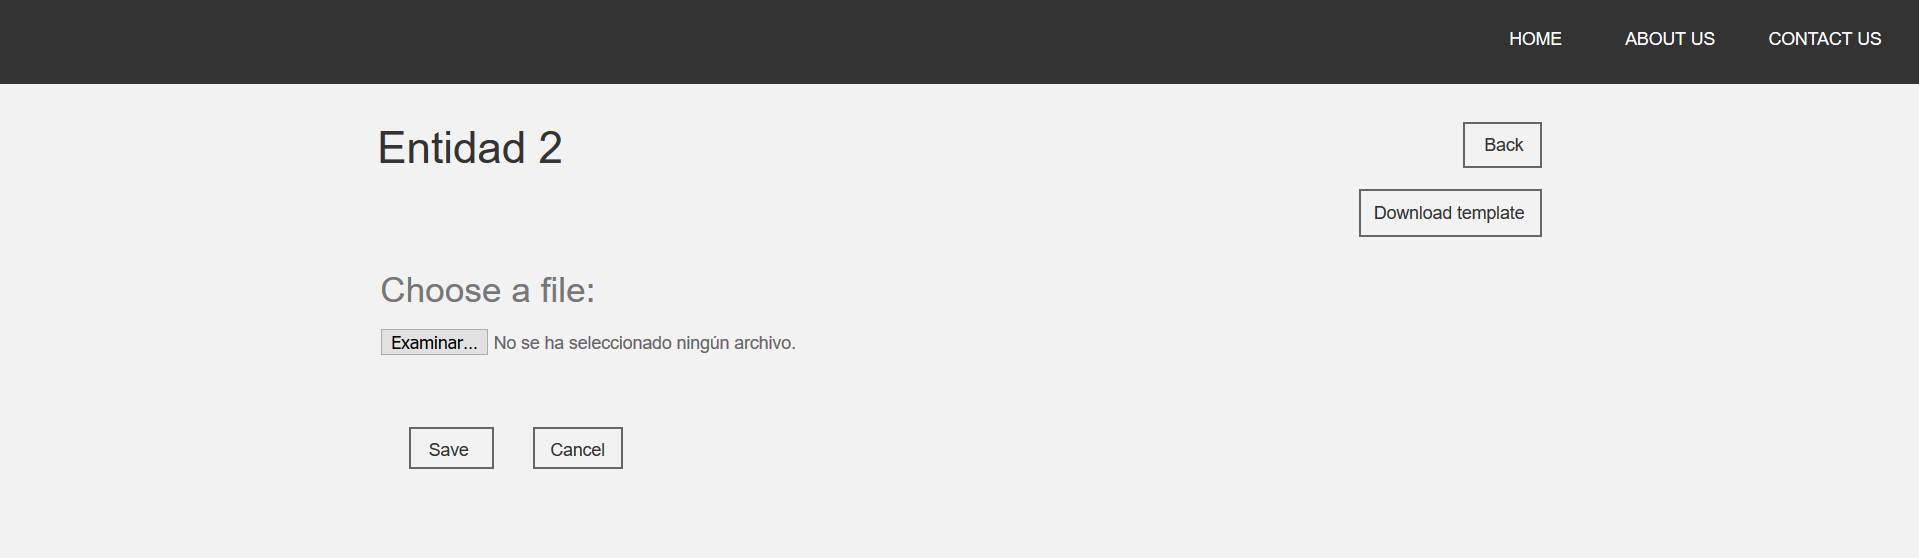
\includegraphics[width=1\textwidth]{/anexos/Diseno/Mockups/entidadExcel}
	\caption{Mockup: Administración de entidades mediante hoja de cálculo.}
	\label{img:entidadExcel}
\end{figure}

%RESULTADO FINAL:

\begin{figure}[h]
	\centering
	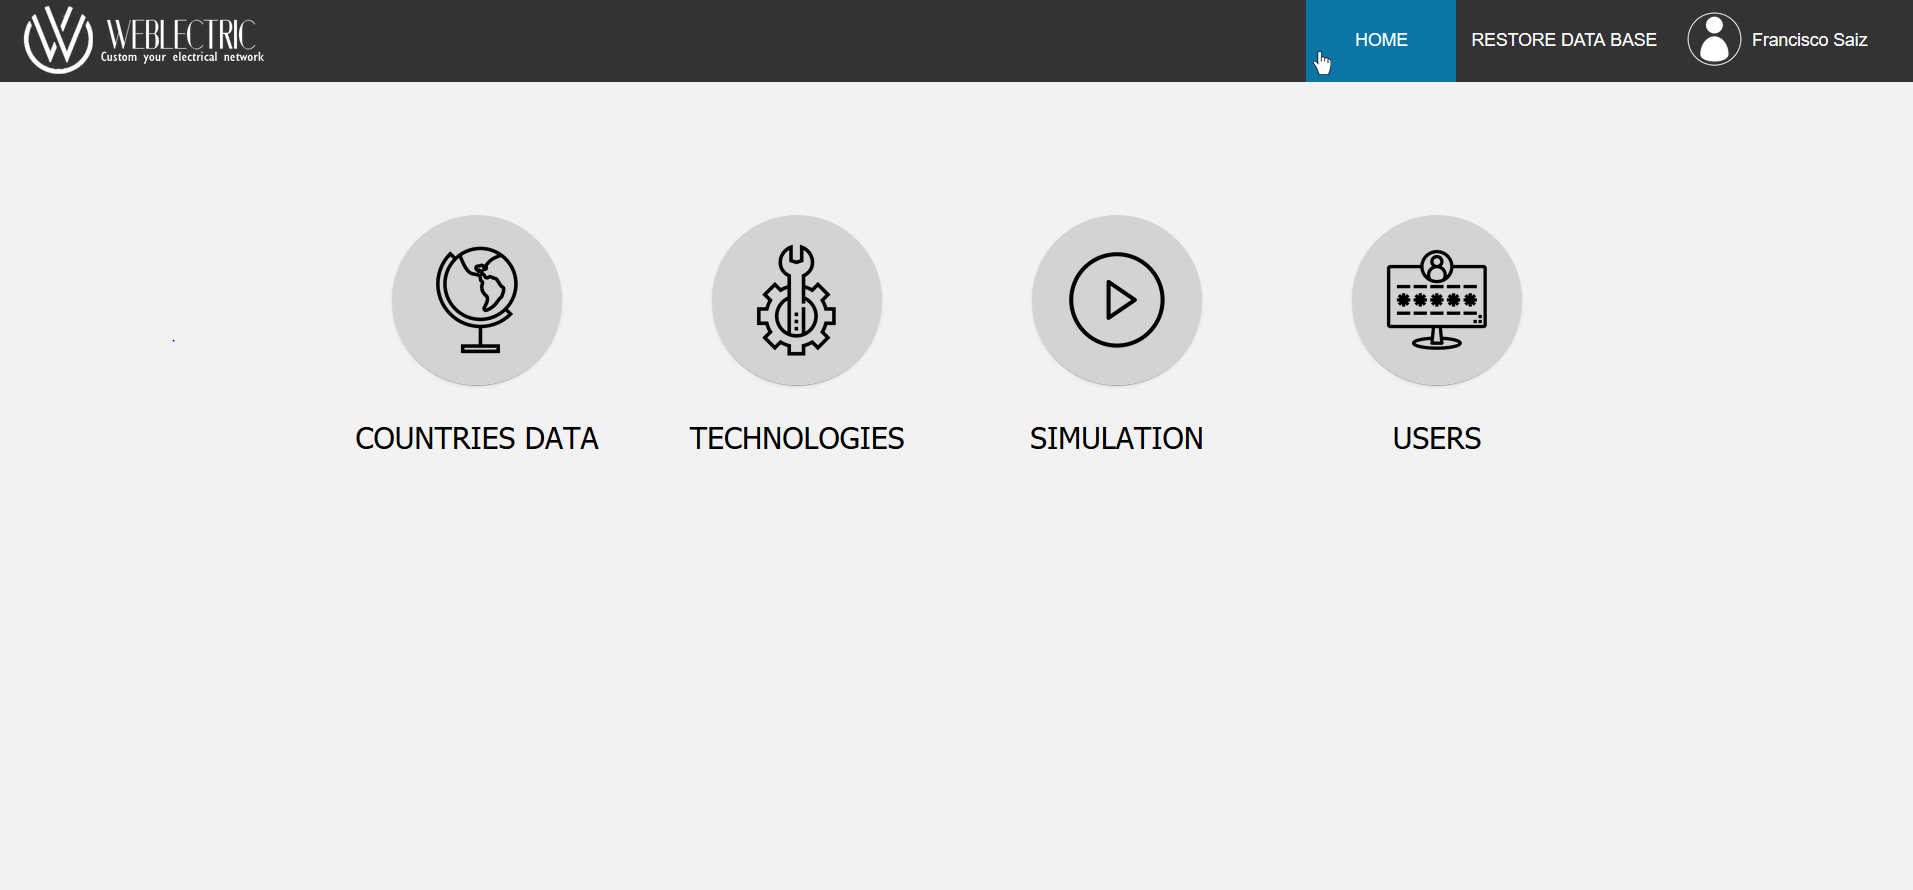
\includegraphics[width=1\textwidth]{/anexos/Diseno/Mockups/Flayout}
	\caption{Resultado final: Plantilla común a todas las vistas.}
	\label{img:Flayout}
\end{figure}

\begin{figure}[h]
	\centering
	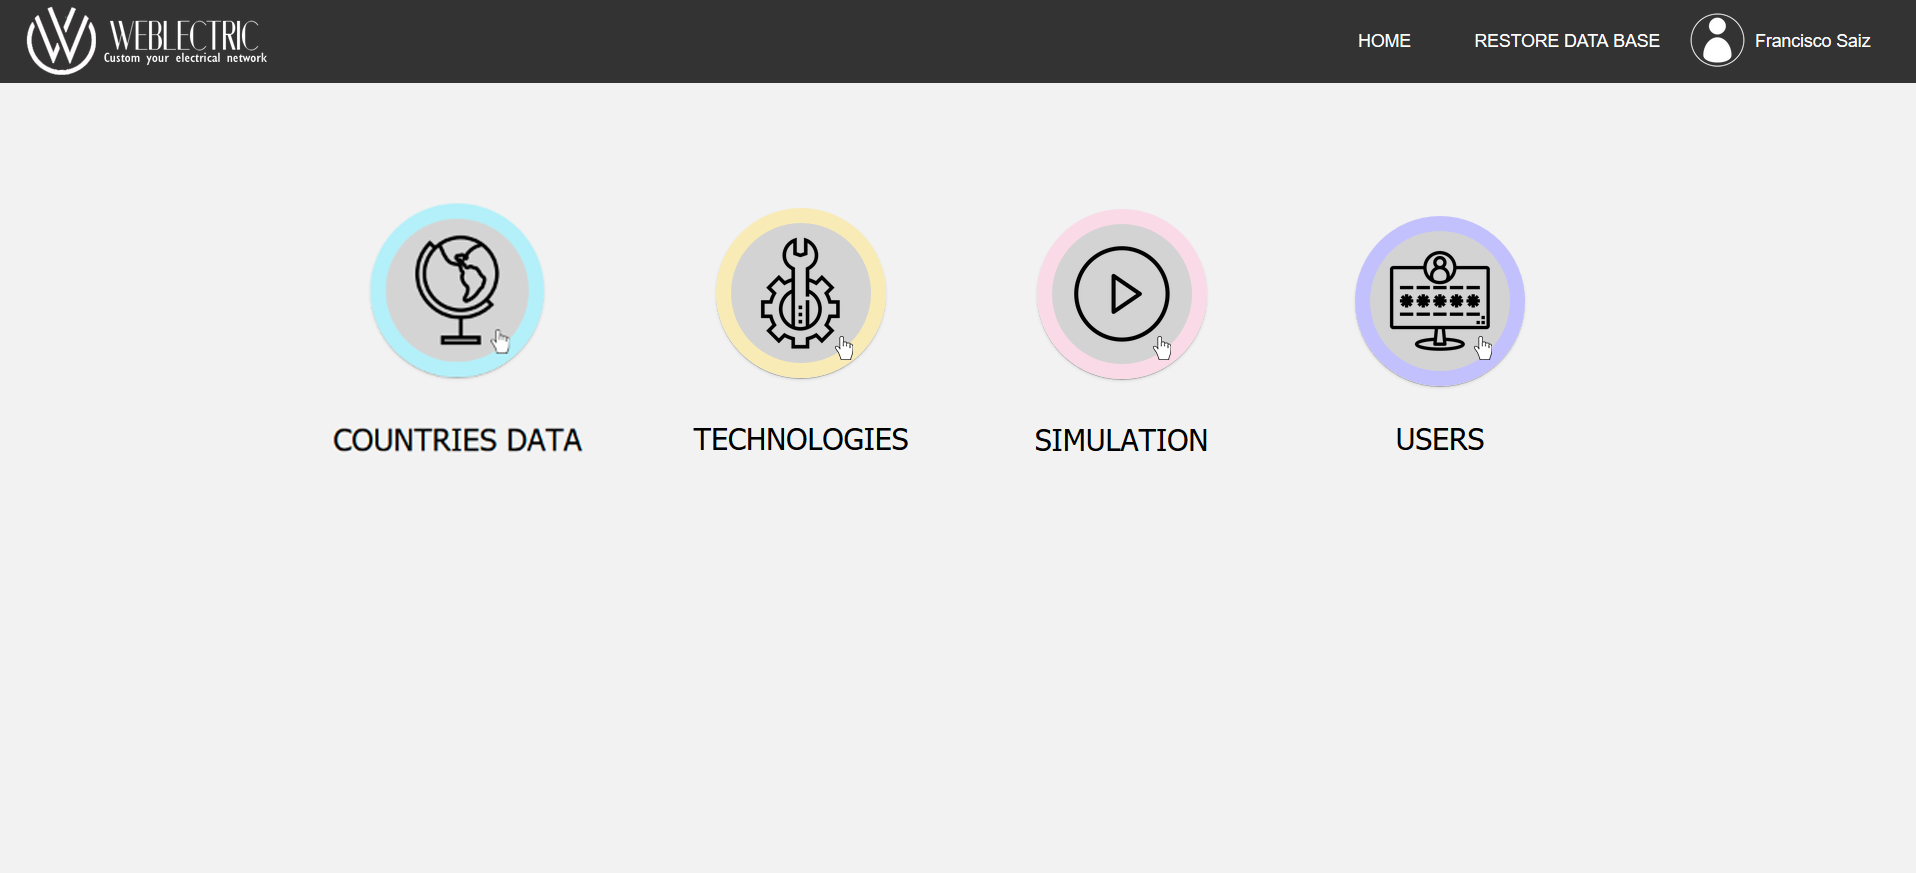
\includegraphics[width=1\textwidth]{/anexos/Diseno/Mockups/Fhome}
	\caption{Resultado final: Pantalla principal.}
	\label{img:Fhome}
\end{figure}

\begin{figure}[h]
	\centering
	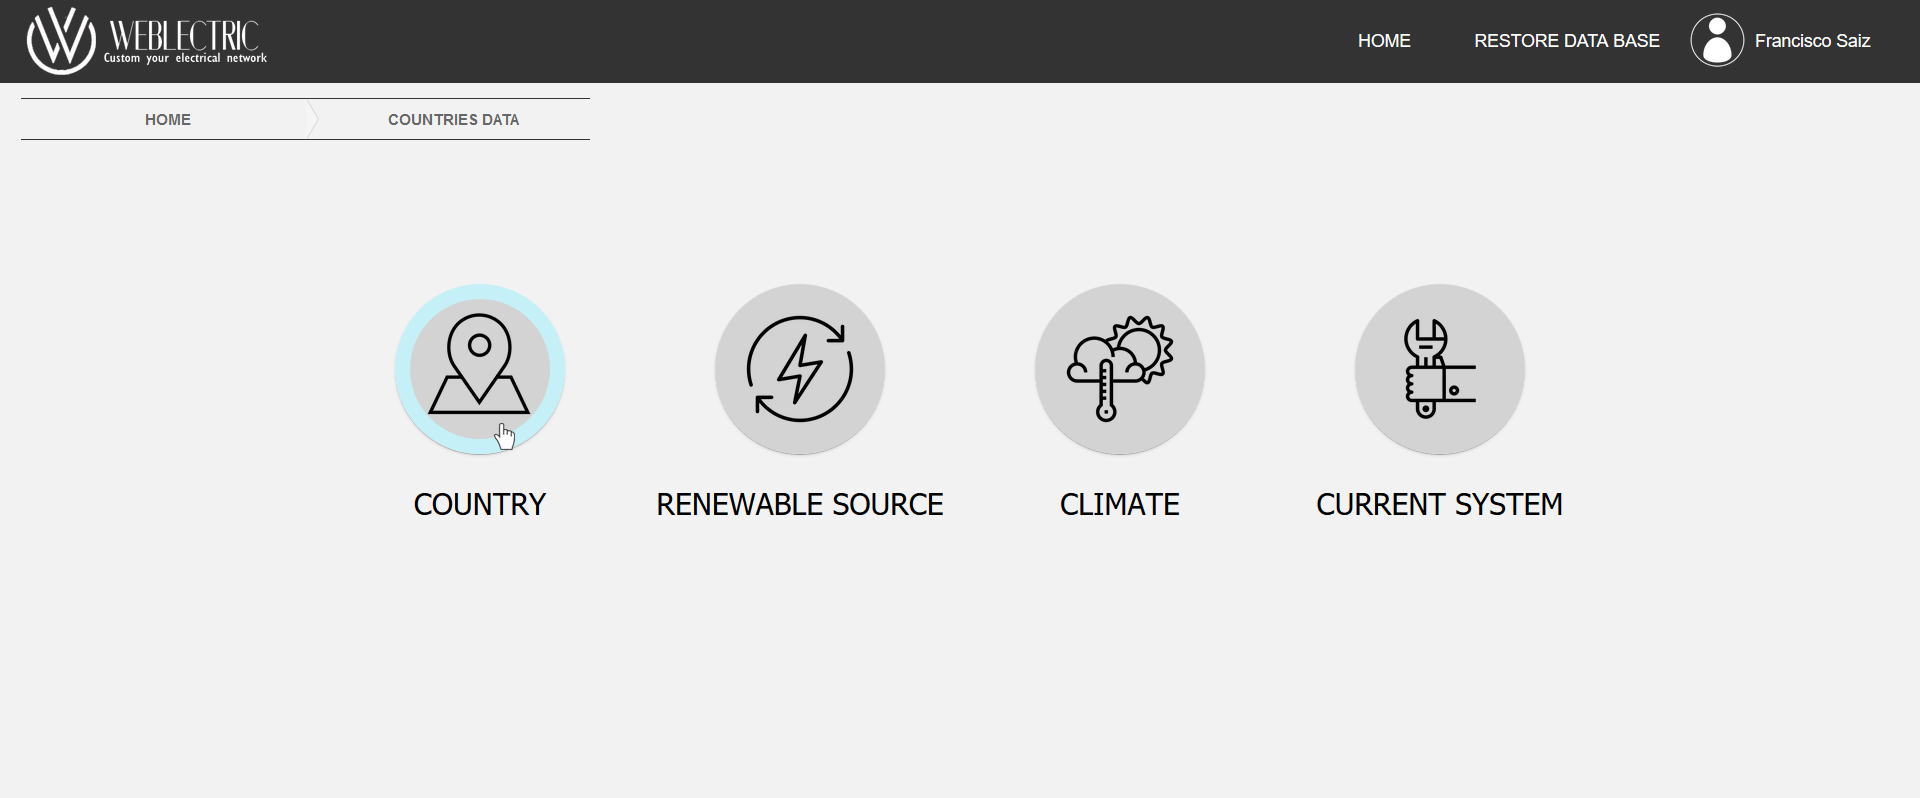
\includegraphics[width=1\textwidth]{/anexos/Diseno/Mockups/Fcountries}
	\caption{Resultado final: Pantalla países.}
	\label{img:Fcountries}
\end{figure}

\begin{figure}[h]
	\centering
	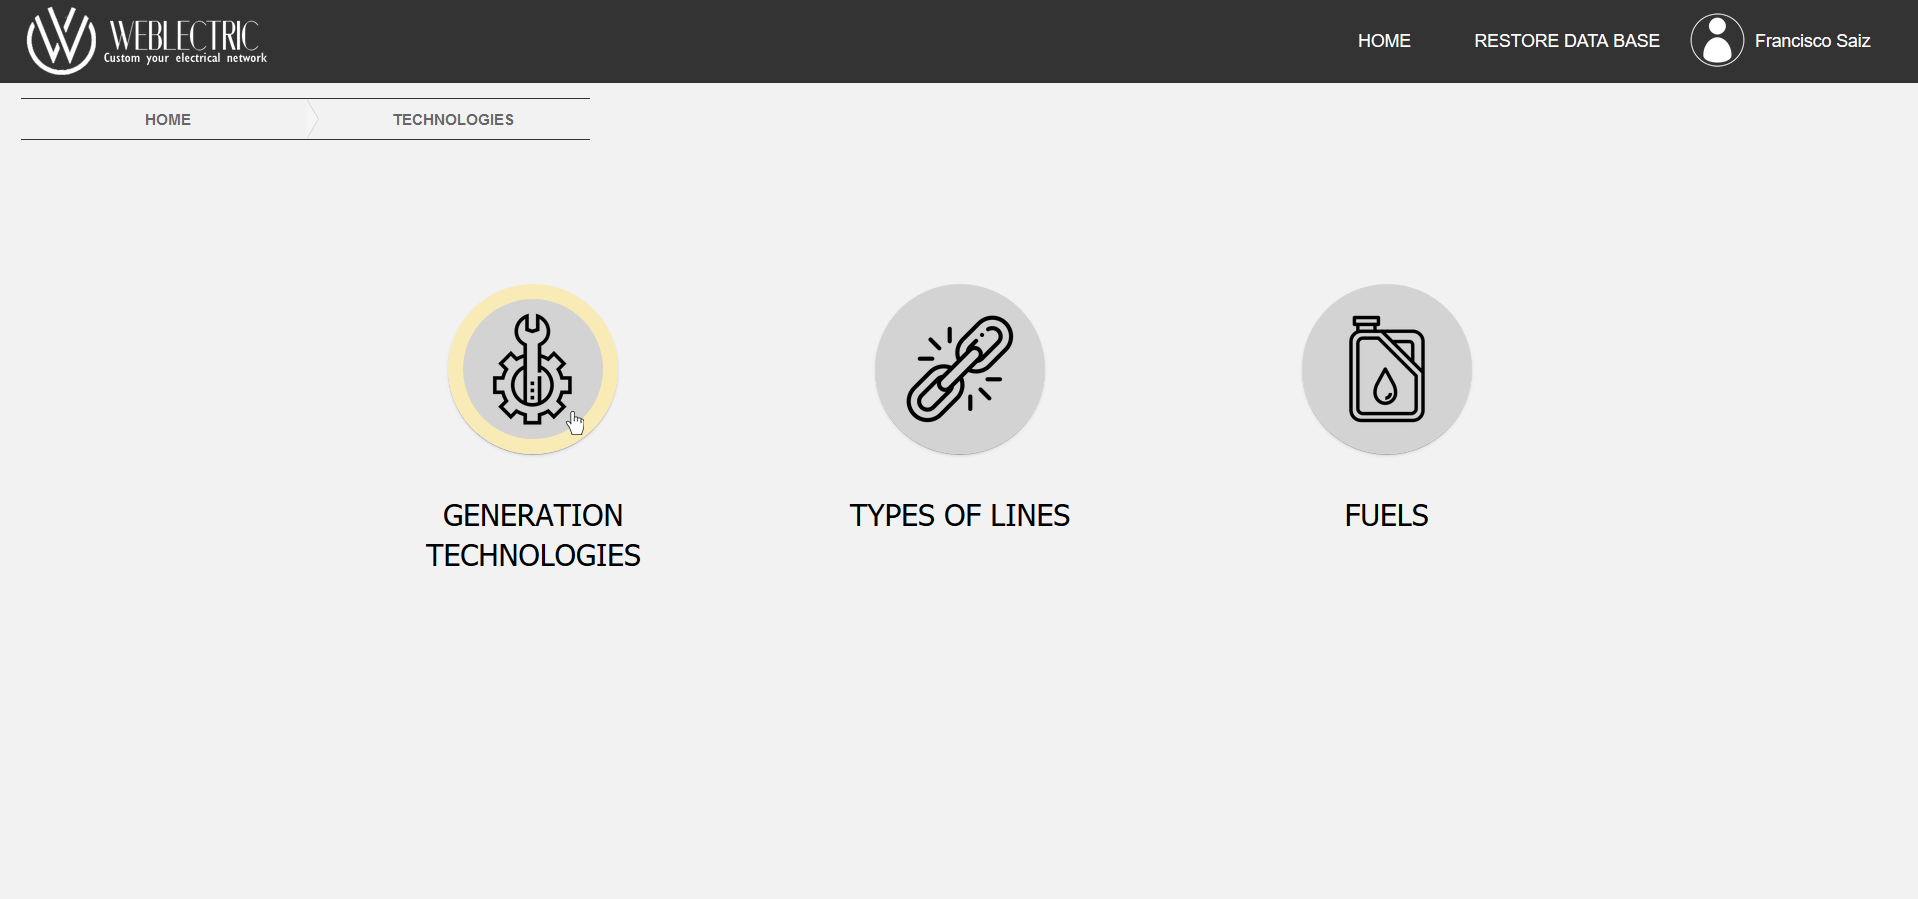
\includegraphics[width=1\textwidth]{/anexos/Diseno/Mockups/Ftechnologies}
	\caption{Resultado final: Pantalla tecnologías.}
	\label{img:Ftechnologies}
\end{figure}

\begin{figure}[h]
	\centering
	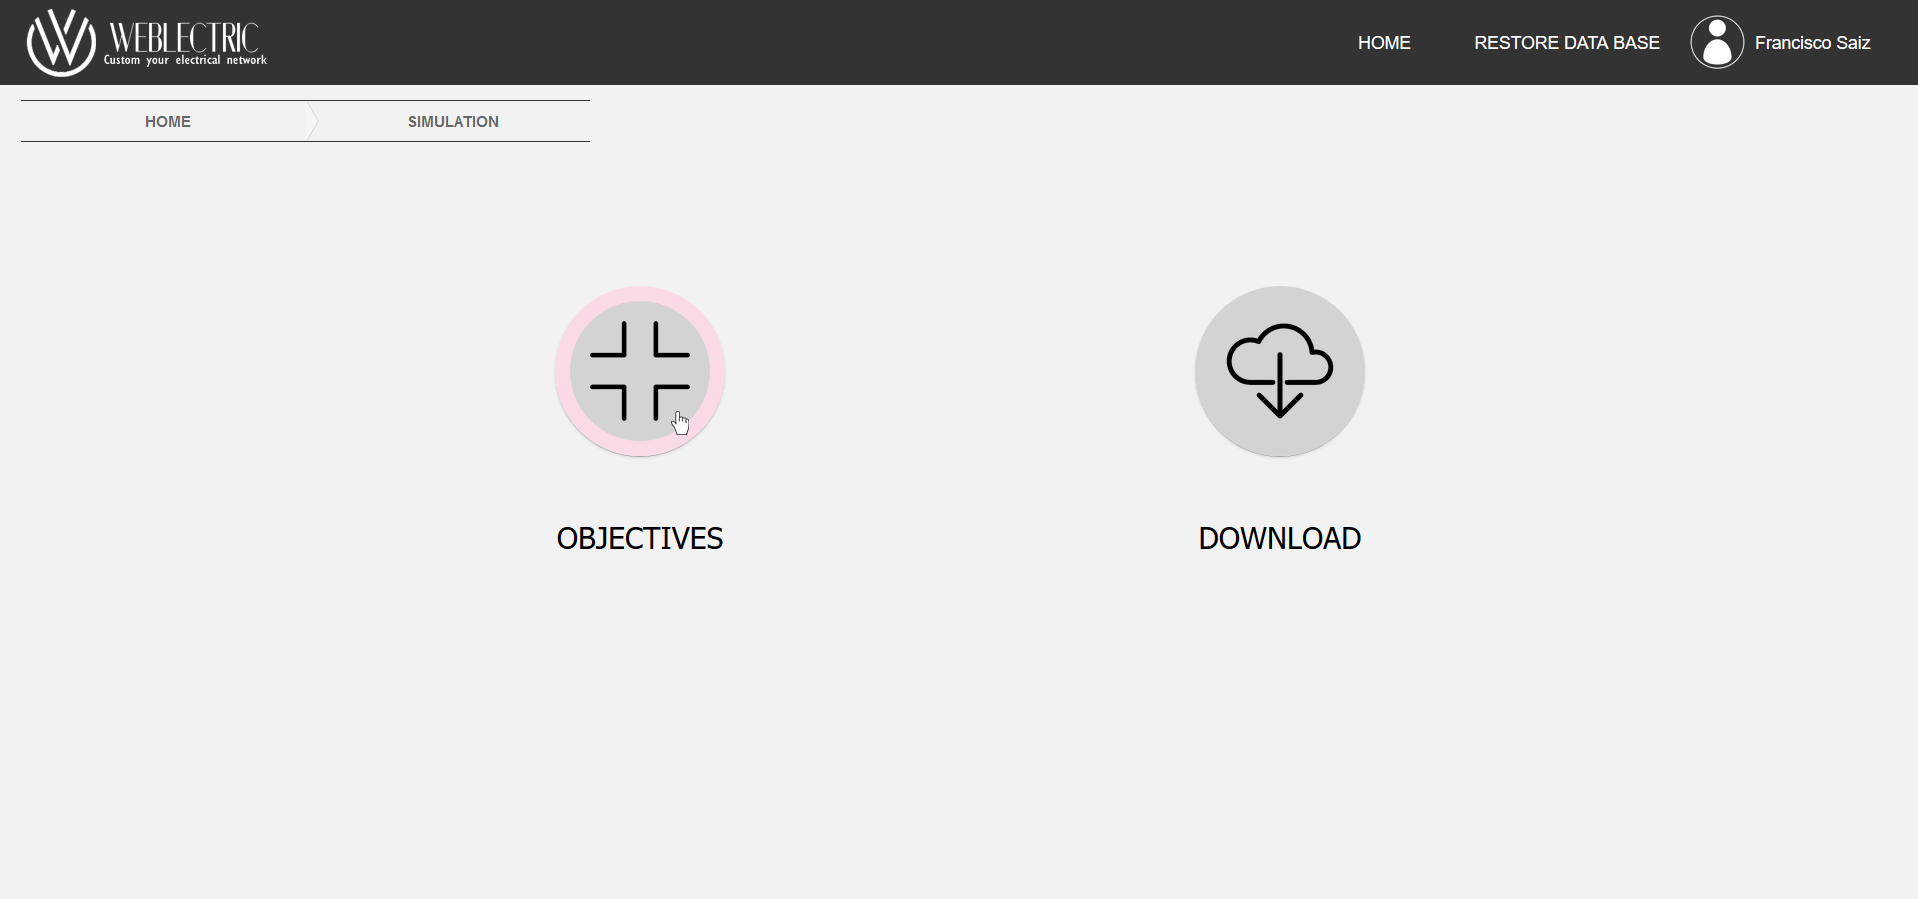
\includegraphics[width=1\textwidth]{/anexos/Diseno/Mockups/Fsimulation}
	\caption{Resultado final: Pantalla simulación.}
	\label{img:Fsimulation}
\end{figure}

\begin{figure}[h]
	\centering
	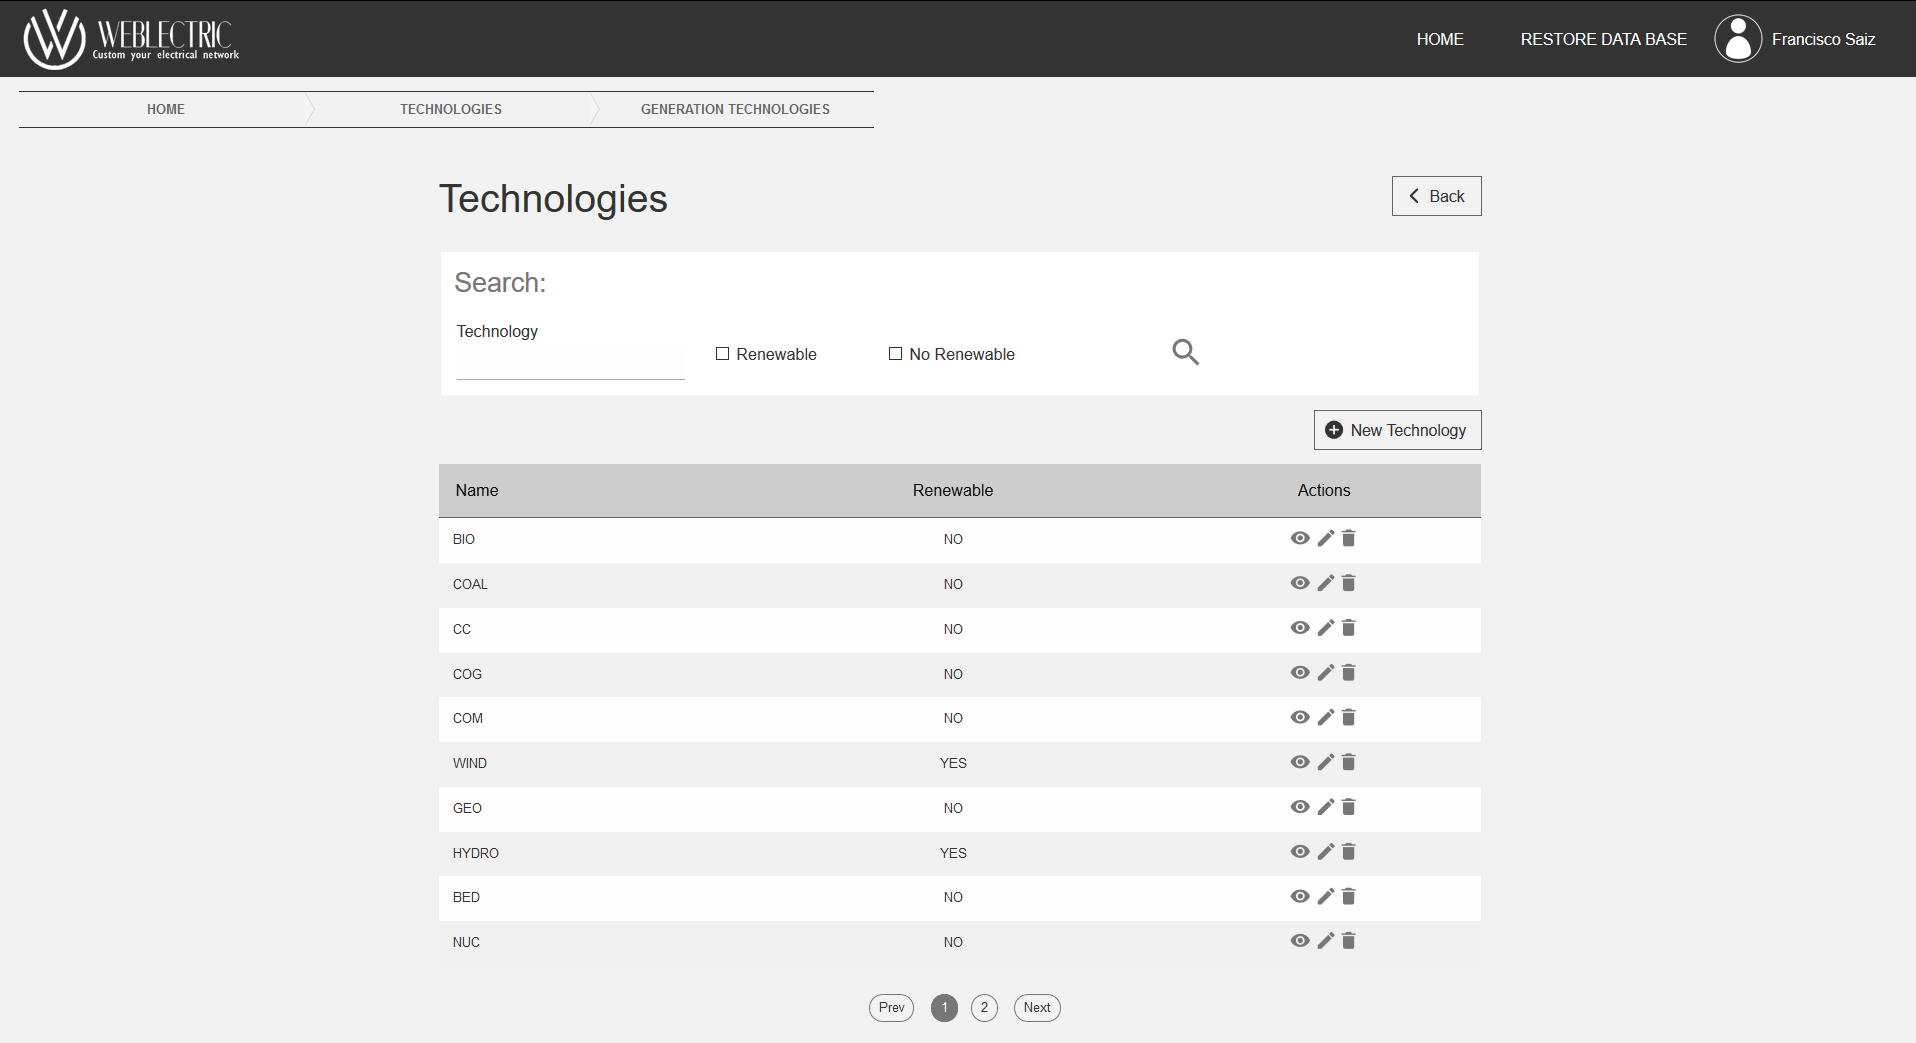
\includegraphics[width=1\textwidth]{/anexos/Diseno/Mockups/FentidadHome}
	\caption{Resultado final: Pantalla principal de la entidad 1.}
	\label{img:FentidadHome}
\end{figure}

\begin{figure}[h]
	\centering
	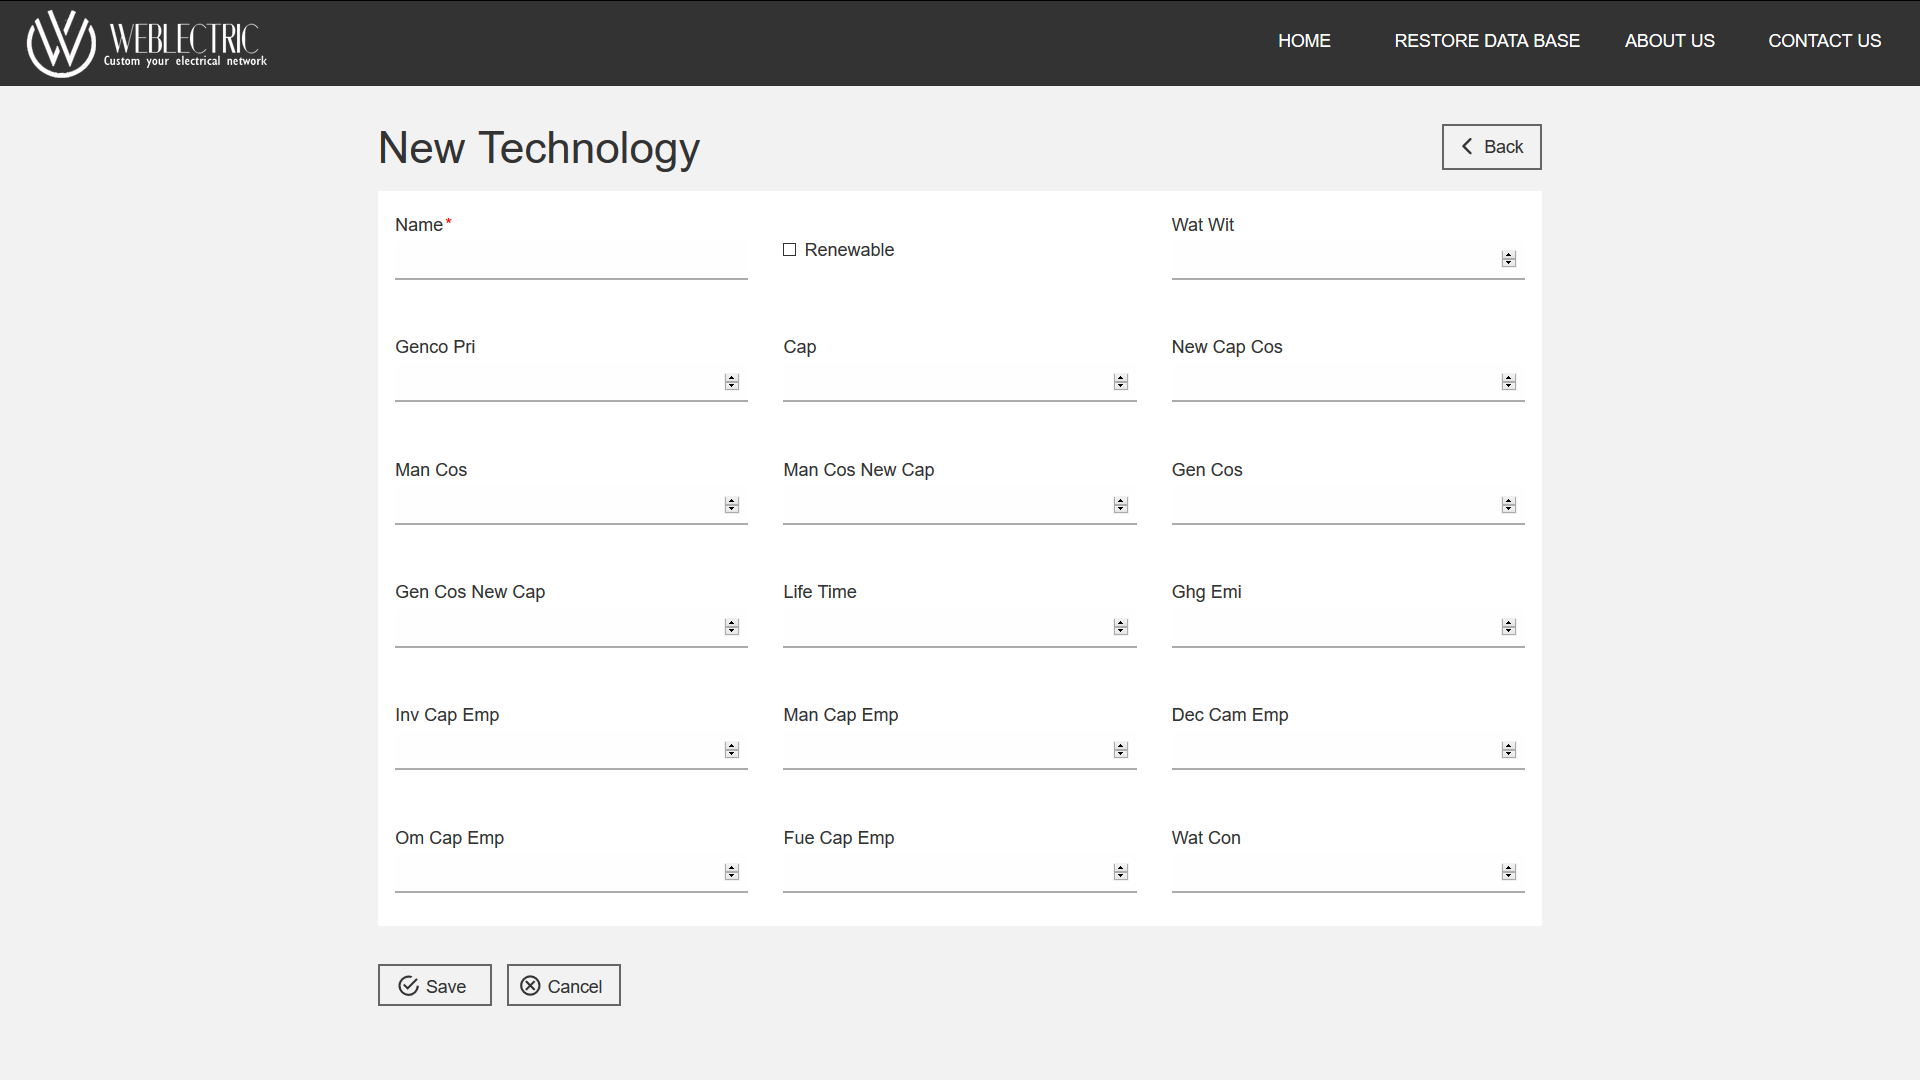
\includegraphics[width=1\textwidth]{/anexos/Diseno/Mockups/FentidadNew}
	\caption{Resultado final: Alta de un elemento.}
	\label{img:FentidadNew}
\end{figure}

\begin{figure}[h]
	\centering
	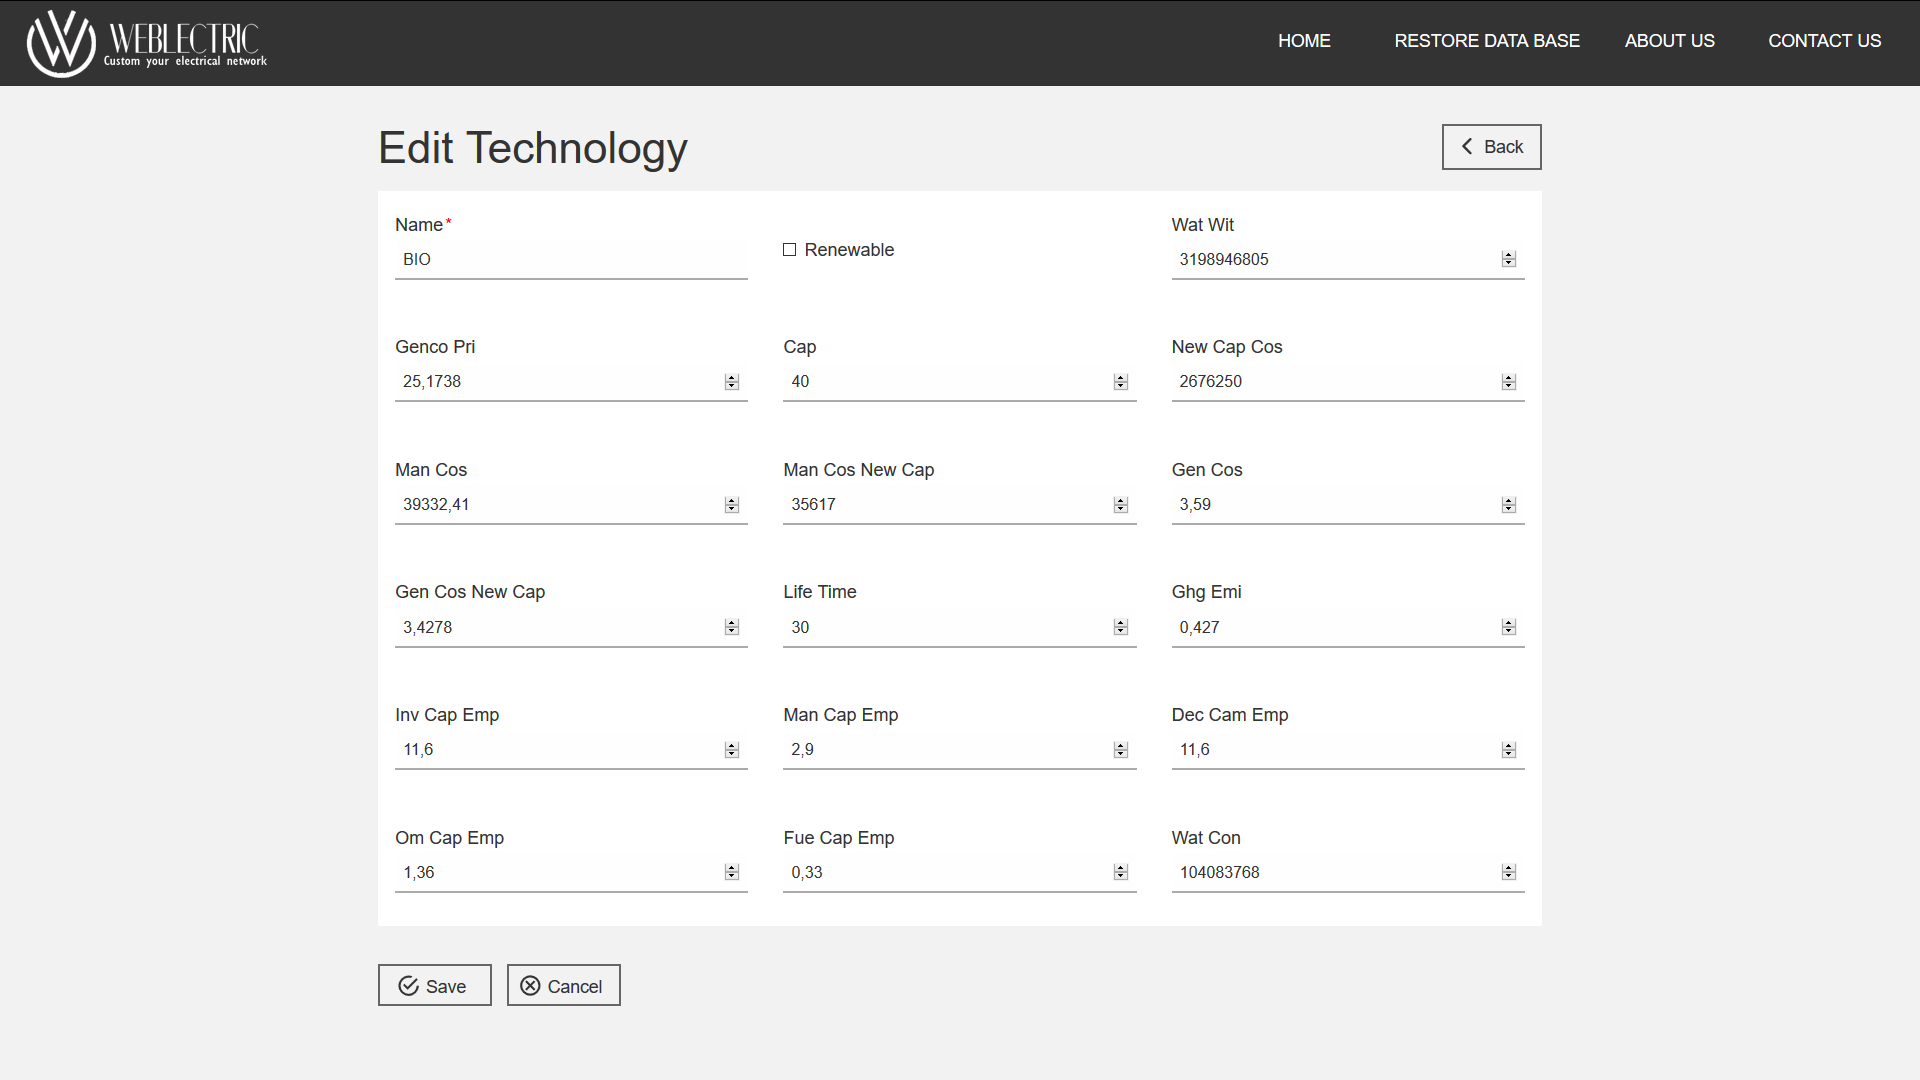
\includegraphics[width=1\textwidth]{/anexos/Diseno/Mockups/FentidadEdit}
	\caption{Resultado final: Edición de un elemento.}
	\label{img:FentidadEdit}
\end{figure}

\begin{figure}[h]
	\centering
	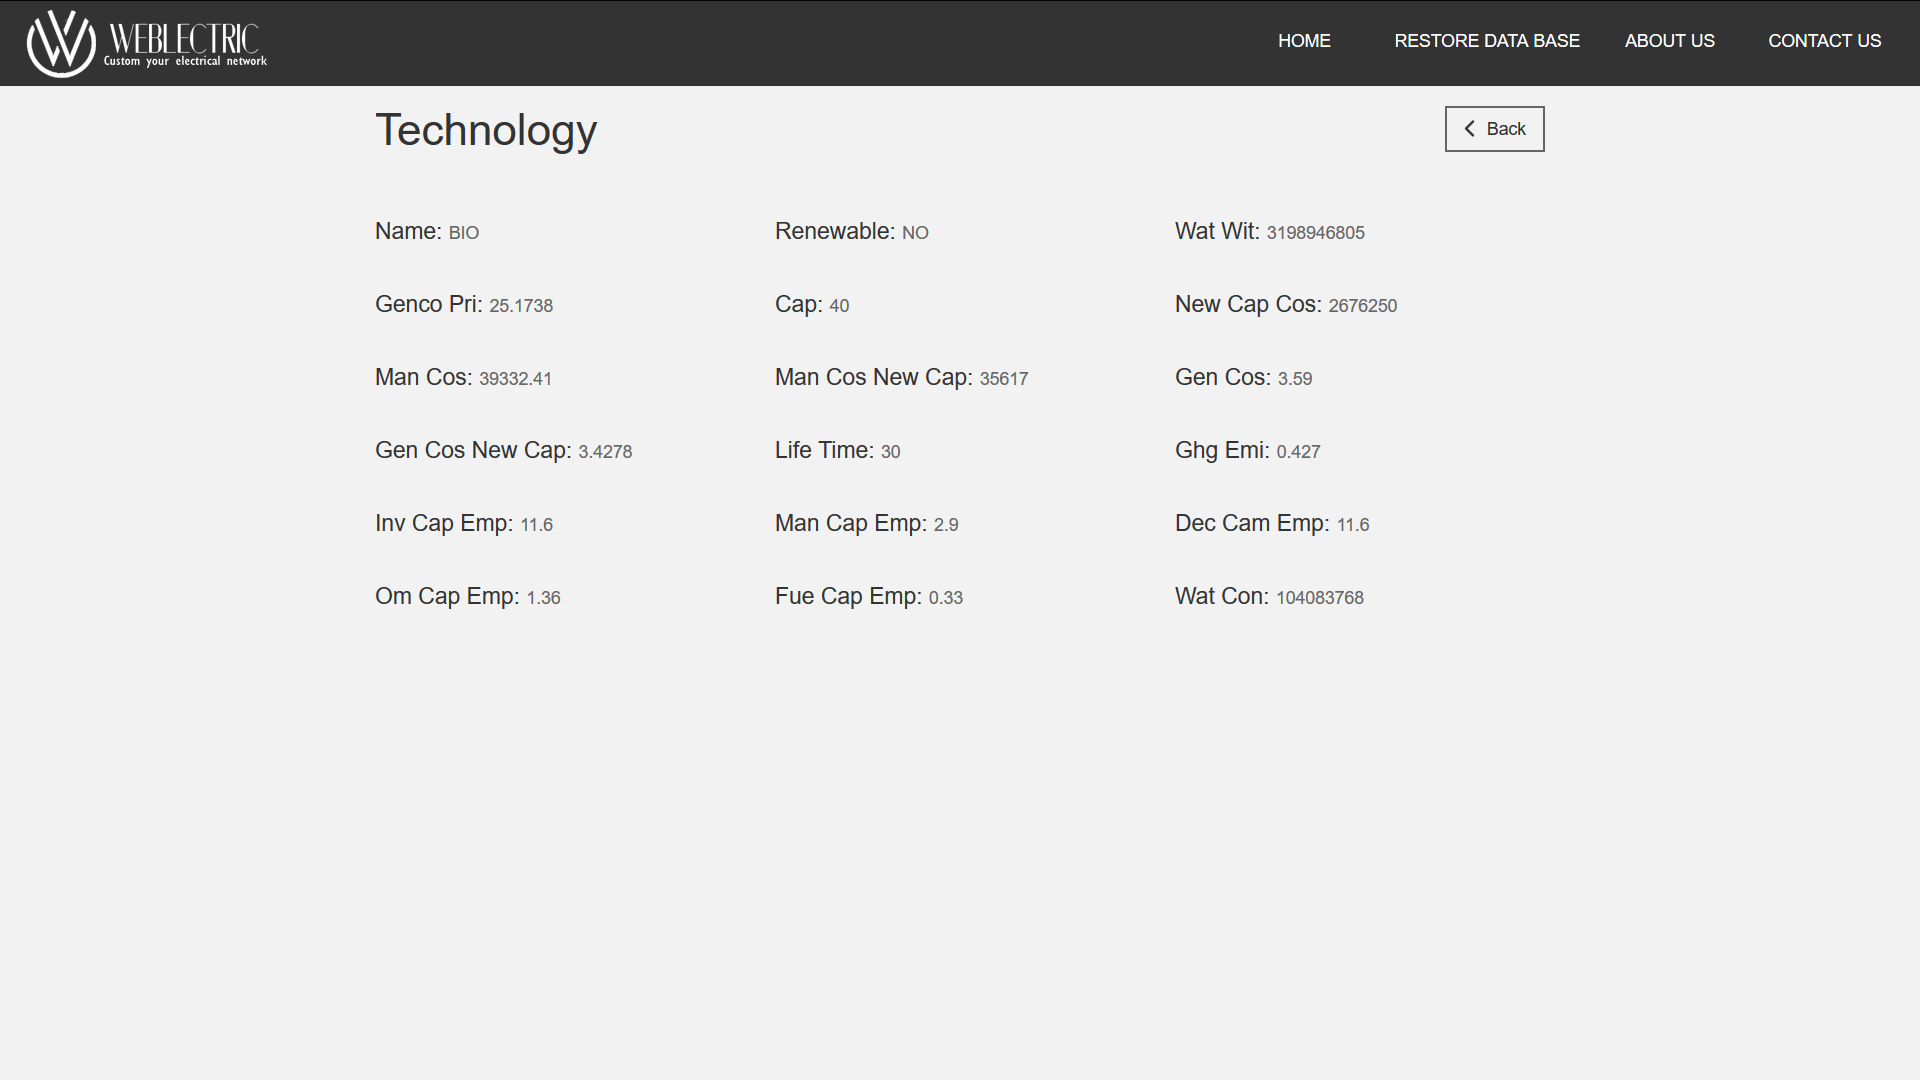
\includegraphics[width=1\textwidth]{/anexos/Diseno/Mockups/FentidadView}
	\caption{Resultado final: Visualización completa de un elemento.}
	\label{img:FentidadView}
\end{figure}

\begin{figure}[h]
	\centering
	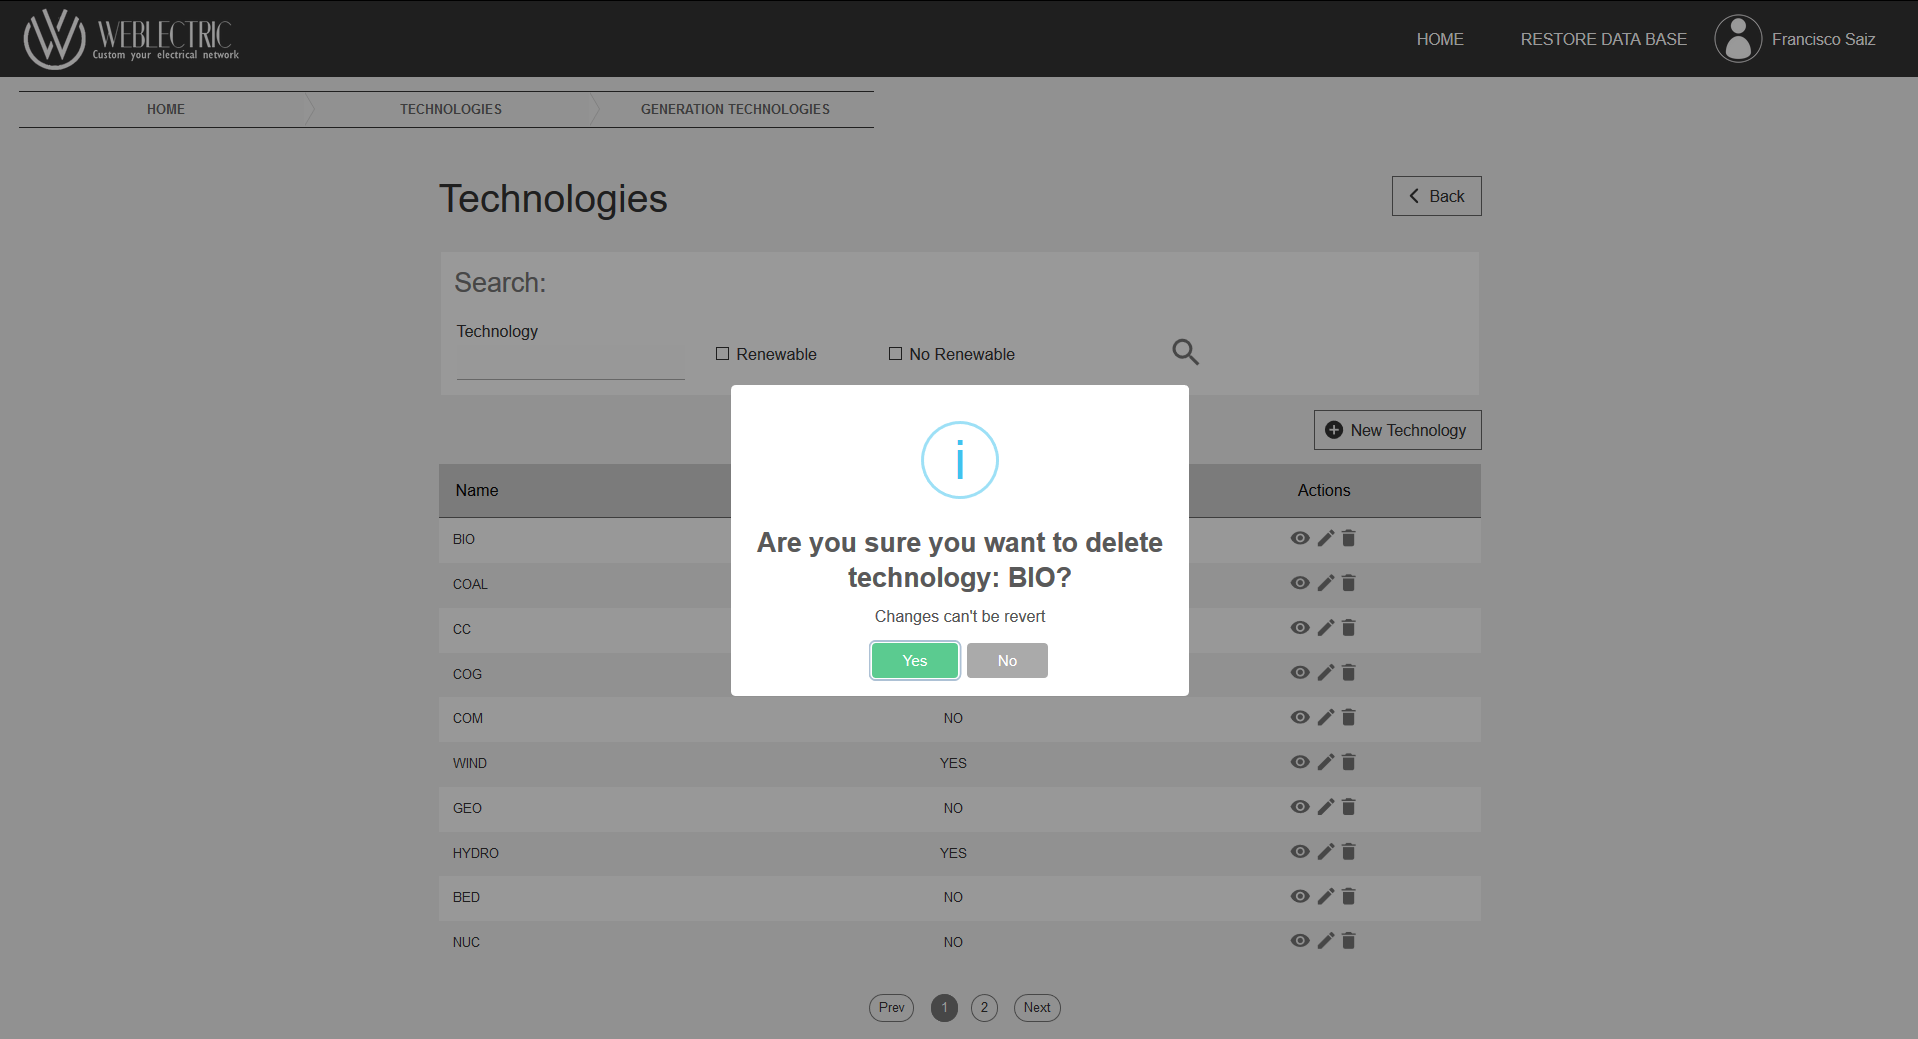
\includegraphics[width=1\textwidth]{/anexos/Diseno/Mockups/FentidadDelete}
	\caption{Resultado final: Mensaje de confirmación al eliminar un elemento.}
	\label{img:FentidadDelete}
\end{figure}

\begin{figure}[h]
	\centering
	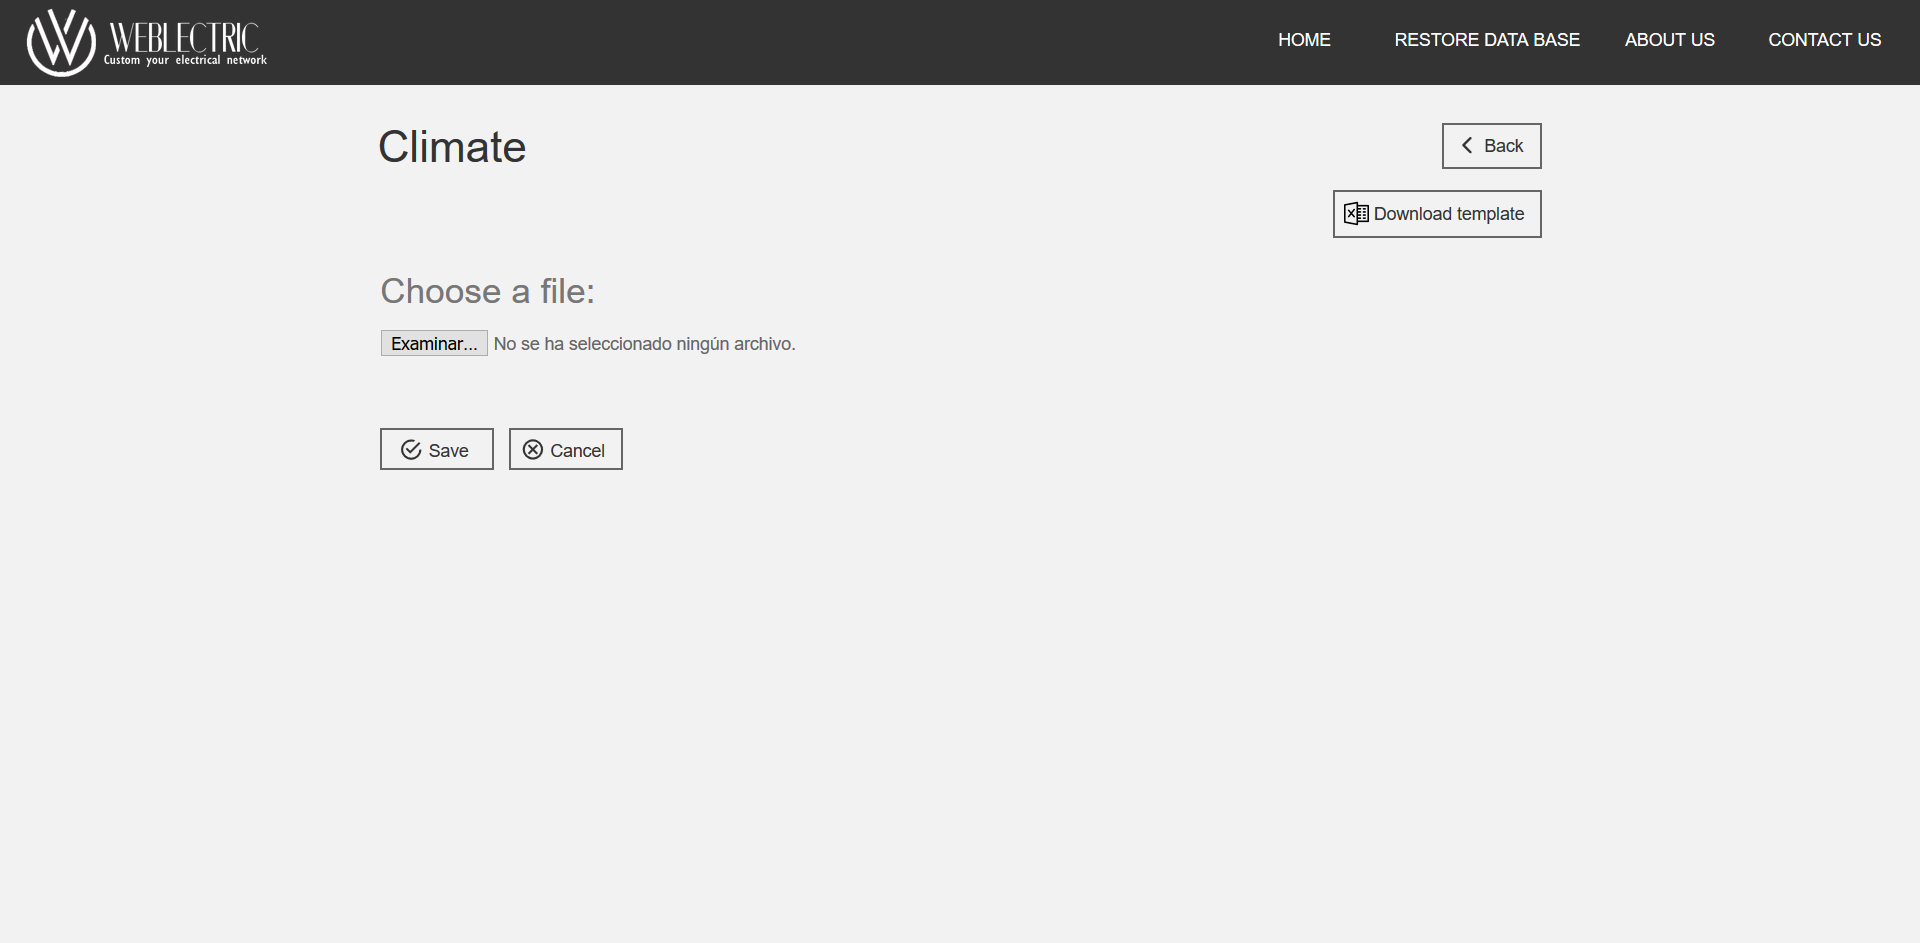
\includegraphics[width=1\textwidth]{/anexos/Diseno/Mockups/FentidadExcel}
	\caption{Resultado final: Administración de entidades mediante hoja de cálculo.}
	\label{img:FentidadExcel}
\end{figure}